%%%%%%%%%%%%%%%%%%%%%%%%%%%%%%%%%%%%%%%%%
% Masters/Doctoral Thesis
% LaTeX Template
% Version 2.5 (27/8/17)
%
% This template was downloaded from:
% http://www.LaTeXTemplates.com
%
% Version 2.x major modifications by:
% Vel (vel@latextemplates.com)
%
% This template is based on a template by:
% Steve Gunn (http://users.ecs.soton.ac.uk/srg/softwaretools/document/templates/)
% Sunil Patel (http://www.sunilpatel.co.uk/thesis-template/)
%
% Template license:
% CC BY-NC-SA 3.0 (http://creativecommons.org/licenses/by-nc-sa/3.0/)
%
%%%%%%%%%%%%%%%%%%%%%%%%%%%%%%%%%%%%%%%%%

%----------------------------------------------------------------------------------------
%	PACKAGES AND OTHER DOCUMENT CONFIGURATIONS
%----------------------------------------------------------------------------------------

\documentclass[
11pt, % The default document font size, options: 10pt, 11pt, 12pt
oneside, % Two side (alternating margins) for binding by default, uncomment to switch to one side
english, % ngerman for German
singlespacing, %singlespacing Single line spacing, alternatives: onehalfspacing or doublespacing
%draft, % Uncomment to enable draft mode (no pictures, no links, overfull hboxes indicated)
%nolistspacing, % If the document is onehalfspacing or doublespacing, uncomment this to set spacing in lists to single
%liststotoc, % Uncomment to add the list of figures/tables/etc to the table of contents
%toctotoc, % Uncomment to add the main table of contents to the table of contents
parskip, % Uncomment to add space between paragraphs
%nohyperref, % Uncomment to not load the hyperref package
headsepline, % Uncomment to get a line under the header
%chapterinoneline, % Uncomment to place the chapter title next to the number on one line
%consistentlayout, % Uncomment to change the layout of the declaration, abstract and acknowledgements pages to match the default layout
]{MastersDoctoralThesis} % The class file specifying the document structure

\usepackage[utf8]{inputenc} % Required for inputting international characters
\usepackage[T1]{fontenc} % Output font encoding for international characters

\usepackage{mathpazo} % Use the Palatino font by default

\usepackage[backend=bibtex,style=authoryear,natbib=true]{biblatex} % Use the bibtex backend with the authoryear citation style (which resembles APA)

\addbibresource{example.bib} % The filename of the bibliography

\usepackage[autostyle=true]{csquotes} % Required to generate language-dependent quotes in the bibliography

\usepackage[labelfont=bf]{caption}
\captionsetup{width=0.8\textwidth}
\usepackage{enumitem}

%\usepackage{ragged2e}%for \justify


%----------------------------------------------------------------------------------------
%	MARGIN SETTINGS
%----------------------------------------------------------------------------------------

\geometry{
	paper=a4paper, % Change to letterpaper for US letter
	inner=2.5cm, % Inner margin
	outer=3.8cm, % Outer margin
	bindingoffset=.5cm, % Binding offset
	top=1.5cm, % Top margin
	bottom=1.5cm, % Bottom margin
	%showframe, % Uncomment to show how the type block is set on the page
}

%----------------------------------------------------------------------------------------
%	THESIS INFORMATION
%----------------------------------------------------------------------------------------

\thesistitle{Optical Flow, Helmholtz Decomposition and Autoencoders for the Characterization of Slow Waves} % Your thesis title, this is used in the title and abstract, print it elsewhere with \ttitle
\supervisor{Dr. Dominik \textsc{Jüstel}} % Your supervisor's name, this is used in the title page, print it elsewhere with \supname
\examiner{Prof. Peter König} % Your examiner's name, this is not currently used anywhere in the template, print it elsewhere with \examname
\degree{Master of Science} % Your degree name, this is used in the title page and abstract, print it elsewhere with \degreename
\author{Michael \textsc{Gerstenberger}} % Your name, this is used in the title page and abstract, print it elsewhere with \authorname
\addresses{} % Your address, this is not currently used anywhere in the template, print it elsewhere with \addressname

\subject{Cognitive Science} % Your subject area, this is not currently used anywhere in the template, print it elsewhere with \subjectname
\keywords{} % Keywords for your thesis, this is not currently used anywhere in the template, print it elsewhere with \keywordnames
\university{\href{http://www.uos.com}{Osnabrück University}} % Your university's name and URL, this is used in the title page and abstract, print it elsewhere with \univname
\department{\href{http://ikw.uos.com}{Institute for Cognitive Science}} % Your department's name and URL, this is used in the title page and abstract, print it elsewhere with \deptname
\group{\href{http://ikw.uos.de/research_groups/neurobiopsychology}{Neurobiopsychology Group}} % Your research group's name and URL, this is used in the title page, print it elsewhere with \groupname
\faculty{\href{http://uos.de/en/university/schools-and-research-facilities/school-of-human-sciences/}{School of Human Sciences}} % Your faculty's name and URL, this is used in the title page and abstract, print it elsewhere with \facname

\AtBeginDocument{
\hypersetup{pdftitle=\ttitle} % Set the PDF's title to your title
\hypersetup{pdfauthor=\authorname} % Set the PDF's author to your name
\hypersetup{pdfkeywords=\keywordnames} % Set the PDF's keywords to your keywords
}

\begin{document}

\frontmatter % Use roman page numbering style (i, ii, iii, iv...) for the pre-content pages

\pagestyle{plain} % Default to the plain heading style until the thesis style is called for the body content

%----------------------------------------------------------------------------------------
%	TITLE PAGE
%----------------------------------------------------------------------------------------

\begin{titlepage}
\begin{center}

\vspace*{.06\textheight}
{\scshape\LARGE \univname\par}\vspace{1.5cm} % University name
\textsc{\Large Master Thesis}\\[0.5cm] % Thesis type

\HRule \\[0.4cm] % Horizontal line
{\fontsize{16}{18}\selectfont \bfseries \ttitle\par}\vspace{0.4cm}% Thesis title
{\fontsize{11}{10}\selectfont  A new approach for temporospatial pattern detection in neuroimaging}% Thesis title
\\
\HRule \\[1.5cm] % Horizontal line

\begin{minipage}[t]{0.4\textwidth}
\begin{flushleft} \large
\emph{Author:}\\
{\authorname} % Author name - remove the \href bracket to remove the link
\end{flushleft}
\end{minipage}
\begin{minipage}[t]{0.4\textwidth}
\begin{flushright} \large
\emph{Supervisors:} \\
Dr. Dominik Jüstel
\\Prof. Peter König
\end{flushright}
\end{minipage}\\[2cm]

\vfill

\large \textit{A thesis submitted in fulfillment of the requirements\\ for the degree of \degreename}\\[0.3cm] % University requirement text
\textit{in the}\\[0.4cm]
\groupname\\\deptname\\[2cm] % Research group name and department name

\vfill

\large \textit{In cooperation with IBMI and ICI at Helmholtz Zentrum Munich}\\[0.1cm] % University requirement text
{\large \today}\\[4cm] % Date
%\includegraphics{Logo} % University/department logo - uncomment to place it

\vfill
\end{center}
\end{titlepage}

%----------------------------------------------------------------------------------------
%	DECLARATION PAGE
%----------------------------------------------------------------------------------------

\begin{declaration}
\addchaptertocentry{\authorshipname} % Add the declaration to the table of contents
\noindent I, \authorname, declare that this thesis titled, \enquote{\ttitle} and the work presented in it are my own. I confirm that:

\begin{itemize}
\item This work was done wholly or mainly while in candidature for a research degree at this University.
\item Where any part of this thesis has previously been submitted for a degree or any other qualification at this University or any other institution, this has been clearly stated.
\item Where I have consulted the published work of others, this is always clearly attributed.
\item Where I have quoted from the work of others, the source is always given. With the exception of such quotations, this thesis is entirely my own work.
\item I have acknowledged all main sources of help.
\item Where the thesis is based on work done by myself jointly with others, I have made clear exactly what was done by others and what I have contributed myself.\\
\end{itemize}

\noindent Signed:\\
\rule[0.5em]{25em}{0.5pt} % This prints a line for the signature

\noindent Date:\\
\rule[0.5em]{25em}{0.5pt} % This prints a line to write the date
\end{declaration}

\cleardoublepage

%----------------------------------------------------------------------------------------
%	ABSTRACT PAGE
%----------------------------------------------------------------------------------------

\begin{abstract}
\addchaptertocentry{\abstractname} % Add the abstract to the table of contents

Neural signal transduction at different levels of alertness occurs in distinct shapes \parencite{eger1981isoflurane}. One may observe stimulus dependent activity during wakefulness but also spontaneous patterns of activation that dominate in stages of deep sleep \parencite{brown2012control}. Similarly, fast neuronal firing is replaced by slow, traveling waves of activation during anaesthesia \parencite{steriade1993novel,celotto2020analysis}. Cortical slow waves can be captured by fluorescence microscopy of GCamp channel activity in transgenic mice at up to 100Hz.\\
Different types of slow waves exist which can incorporate rather localized or more widespread regions of cortex \parencite{bernardi2018local}. Neocortical slow waves are distinguished from delta waves \parencite{steriade1993novel}. In principle, they are thought to occur spontaneously in various regions, however it was also noted that synchrony with somatosensory states and more importantly signals in subcortical structures exists \parencite{stroh2013making}. Neocortico-hippocampal synchrony is related to memory formation \parencite{maingret2016hippocampo}. Recently important differences between cortical sleep slow waves and their counterpart during anaesthesia were identified \parencite{nghiem2018two}. This shows that slow waves represent an important yet highly variable neural phenomenon and indicates that methods are required that allow to systematically distinguish slow waves based on their properties.\\
Townsend and Gong \parencite{townsend2018detection} suggest to characterize temporospatial properties of neural recordings by the detection of patterns in Dense Optical Flow. It shows, however, that the use is accompanied by two challenges: First it shows that focal brightness changes result in sources and sinks in the vector fields. Second successful estimation of Optical Flow is challenged by the quality of the contrast it is applied on. Here it is demonstrated how both can be addressed and Dense Optical Flow used successfully to characterize slow waves. The presented procedure allows for a scale independent split of optogenetic recordings into several segments that include neocortical slow waves. This allows for an event related analysis and the computation of a contrast that is independent from anatomical structures and meets the smoothness requirements of Dense Optical Flow. It is further demonstrated that Helmholtz-Decomposition can be used to distinguish between the effect of local sources of neural activation and global patterns of neural flow. Finally, it is shown how the measured high-level features can be analysed using variational autoencoders. The approach reveals a complex topology of the distribution of different features in latent slow-wave-space. These features include the direction of flow and the distribution of sources, duration and amplitude. It shows that the combination of different types of events differs between stages of anaesthesia.\\
In summary a new technique to characterize slow-waves is presented that can help to improve our understanding of neural processing in the brain under anaesthesia. The use of Optical Flow, Helmholtz-Decomposition and autoencoders to characterize and distinguish different types of slow waves appears promising. It bears potentials to study the relationship between distributions of events and other features including anaesthetics, experimental stimuli or animal behavior.
\end{abstract}
\onehalfspacing % Reset line spacing to 1.5 from here on

%----------------------------------------------------------------------------------------
%	ACKNOWLEDGEMENTS
%----------------------------------------------------------------------------------------

\begin{acknowledgements}
\addchaptertocentry{\acknowledgementname} % Add the acknowledgements to the table of contents
I would like to thank my supervisors for their support of my Master Thesis. Especially I want to thank Silviu Bodea who initiated the project, recorded all the data and made my contribution possible. Special thanks go to him and Prof. Gil Westermeyer of the Institute of Biological and Medical Imaging (IBMI) for the continuous feedback and advice regarding the results and further direction of my work. Besides I want to genuinly thank my first supervisor, Dr. Dominik Juestel for his input regarding the methodological questions and especially for pointing out the benefits of Helmholtz-Decomposition. I truly enjoyed taking part in the meetings of his group at the Institute for Computational Biology (ICI) and appreciate that I gained interesting insights in the work of the other members which gave variety to my work during the global pandemics. Finally I want to thank my second supervisor Prof. Peter König of Osnabrück University especially for his stuctured guidance regarding a cooperation with external partners during the Master Thesis.
\end{acknowledgements}

%----------------------------------------------------------------------------------------
%	LIST OF CONTENTS/FIGURES/TABLES PAGES
%----------------------------------------------------------------------------------------

\tableofcontents % Prints the main table of contents

\listoffigures % Prints the list of figures

%\listoftables % Prints the list of tables

%----------------------------------------------------------------------------------------
%	ABBREVIATIONS
%----------------------------------------------------------------------------------------

\begin{abbreviations}{ll} % Include a list of abbreviations (a table of two columns)

\textbf{EEG} & \ Electroencephalogram\\
\textbf{ECoG} & \ Electrocorticogram\\
\textbf{fMRI} & \ Functional Magnetic Resonance Imaging\\
\textbf{MRI} & \ Magnetic Resonance Imaging\\
\textbf{CT} & \ Computed tomography (X-ray)\\
\textbf{GCaMP} & \ A genetically modulated calcium channel with green flouroscence\\
\textbf{K+} & \ Potassium ions\\
\textbf{Ca2+} & \ Calcium ions\\
\textbf{NMDA} & \ N-Methyl-D-Aspartic-Acid\\
\textbf{GABA} & \ Gamma-Aminobutyric-Acid\\
\textbf{iso} & \ Isoflurane\\
\textbf{ARAS} & \ Ascending reticular activation system\\
\textbf{RMT} & \ Rostral midline thalamic nucleus\\
\textbf{LP} & \ Lateral posterios nucleus of thalamus\\
\textbf{MnPO} & \ Medial nucleus of the preoptic area\\
\textbf{RTN} & \ Reticular thalamic nucleus\\
\textbf{SCN} & \ Suprachismatic nucleus\\
\textbf{VLPO} & \ Ventrolateral nucleus of the preoptic area\\
\textbf{MnPO} & \ Medial nucleus of the preoptic area\\
\textbf{RSD} & \ Retrosplenial Dysgranular\\
\textbf{REM} & \ Rapid eye movement \\
\textbf{RBF} & \ Radial basis function\\
\textbf{CNN} & \ Convolutional neural network\\
\textbf{VAE} & \ Variational Autoencoder\\
\textbf{UNet} & \ Autoencoder with U-shape\\
\textbf{MLP} & \ Multilayer perceptron where all layers are fully connected.\\
\textbf{RELU} & \ Rectified linear units\\





\end{abbreviations}

%----------------------------------------------------------------------------------------
%	THESIS CONTENT - CHAPTERS
%----------------------------------------------------------------------------------------

\mainmatter % Begin numeric (1,2,3...) page numbering

\pagestyle{thesis} % Return the page headers back to the "thesis" style

% Include the chapters of the thesis as separate files from the Chapters folder
% Uncomment the lines as you write the chapters

\onehalfspacing % Set line spacing to 1.5
\fontsize{12}{16}\selectfont

% Chapter 1

\chapter{Introduction} % Main chapter title

\label{Chapter1} % For referencing the chapter elsewhere, use \ref{Chapter1}
%----------------------------------------------------------------------------------------
% Define some commands to keep the formatting separated from the content
\newcommand{\keyword}[1]{\textbf{#1}}
\newcommand{\tabhead}[1]{\textbf{#1}}
\newcommand{\code}[1]{\texttt{#1}}
\newcommand{\file}[1]{\texttt{\bfseries#1}}
\newcommand{\option}[1]{\texttt{\itshape#1}}
%----------------------------------------------------------------------------------------
Anaesthesia inhibits neural activity and alters the signals in the brain. Depending on the dosage of the anaesthetic in use different patterns can be observed \parencite{eger1981isoflurane}. At intermediate concentrations many agents cause propagating low-frequency waves that occur in close succession and manifest as slow oscillations in EEG \parencite{steriade1993novel, eger1981isoflurane}. Similar patterns can be observed during deep sleep. Neocortical slow waves differ in shape and size and with respect to specific temporo-spatial features: Most importantly the source location of recurrent activation, the direction and speed of spread and different sets of functionally connected regions can be observed \parencite{brown2012control}. These features can be measured using modern imaging techniques that capture the fluorescence of genetically modified GCamp channels.\\
The development of new experimental technologies to capture GCamp fluorescence with an increasing temporal resolution of up to 100Hz offers new opportunities for the study of the neural circuitry and dynamic state changes of the brain under anaesthesia. At the same time, they also impose new challenges that result from the complexity of the recorded data. These challenges must be addressed by a well-controlled experiment or suitable approaches for data analysis.\\
Strict experimental control simplifies data processing. Under certain experimental conditions, high amplitude slow waves with a good signal to noise ratio and contrast to the hemodynamic autoflourescence occur in a regular pattern. For ketamine induced anaesthesia (100mg/kg), regular patterns of neocortical slow waves with highly similar shapes, durations and amplitudes occur. This simplifies the separation of events and the subsequent analysis \parencite{celotto2020analysis}. However, such strict control means that the variance of the captured slow waves is highly reduced.\\
More general findings regarding the structure of neocortial slow waves are only possible in less controlled settings. This means, however, that suitable methods for data processing and analysis must be established that are both robust and suitable to capture the dynamics of neocortical slow waves of different shapes and signal strengths.\\
Hence a new approach was developed that allows to distinguish and characterize neocortical slow waves of various shapes and forms. It reveals a complex topology of events and shows how different levels of isoflurane change the way signals travel in the brain. The development was accompanied by two major questions: (1) What are slow waves and (2) how can their temporospatial properties be measured and characterized. To answer the earlier question and provide a working definition for neural slow waves that allows to distinguish different events, relevant slow wave literature was systematically reviewed. To tackle the latter question, it was investigated how Dense Optical Flow can be used to measure the strengths and direction of neural flow and how Helmholtz Decomposition can help to distinguish it from neural sources and areas of extended recurrent activity. As not only features but characteristic patterns are of interest it was further assessed how autoencoders can be used for dimensionality reduction of the measured properties.\\
In the following the results of named literature review are presented first (section \ref{Chapter2}). It shows that anaesthetics change important properties of neurons most prominently their excitability which explains why bistable states of network activity that can be observed in neocortex empirically (see section \ref{effects_of_anaesthesia}). While important differences exist between anaesthesia and sleep, slow waves can be observed in both states. One may distinguish corticothalamic slow waves in the delta range and neocortical slow waves of a duration above one second (see section \ref{slow_waves_anaesthesia_sleep}). The latter kind of slow waves is of main interest here. They are understood as extended periods of recurrent neural activation that manifests as above baseline activity (see section \ref{working_definition}). \\
The methods to analyse slow waves are explained in the second part. First a new approach is presented that allows to track haemoglobin rich blood in vessels of various size. It is shown that high amplitude oscillations result from intracranial blood flow and band-stop filtering can be used to reduce this effect. Second an overview of the processing steps is provided. The procedure of splitting events is reported, then Dense Optical Flow is introduced, and it is demonstrated how Helmholtz Decomposition can be used to distinguish between the effect of local brightness changes and global flow. Subsequently the use of autoencoders for unsupervised characterization of slow waves is discussed and the hyperparameters of the models used are presented. \\
The results of the approach are shown in the third part. First simple statistics regarding the dataset, selected features and the experimental conditions are reported. Then the relationship between properties of waves is summarized for representative events. Finally, the results of the autoencoders are reported. \\
In the last part the findings regarding the methods and the achieved results are discussed. Optical-flow, Helmholtz decomposition and autoencoders are a suitable tool to study slow waves. Feature engineering helps to select relevant and robust features. Optical flow can be used in combination with Helmholtz-Decomposition to distinguish between local sources and global pathways of neural flow. Autoencoders represent an easy-to-use tool for the analysis of high-level features. The results confirm the existence of fundamentally different types of slow waves. The approach allows for a fine-grained distinctions and reveals a complex topology of static and dynamic properties in latent slow wave space.\\

% Chapter Template

\chapter{Slow waves} % Main chapter title

\label{Chapter2} % Change X to a consecutive number; for referencing this chapter elsewhere, use \ref{ChapterX}
\label{review} % For referencing the chapter elsewhere, use \ref{Chapter1}


%----------------------------------------------------------------------------------------
%	SECTION 1
%----------------------------------------------------------------------------------------

\section{Overview: Types, functions and modes of action}
\label{overview_of_functions_and_types}
There is a large body of literature that addresses slow oscillations in the brain. Slow waves in the delta range (0.5-4 Hz) can been identified in electroencephalograms (EEG) in deep sleep and under anaesthesia. Neurons that switch between up and down states in the respective frequency are present in thalamus indicating that this kind of slow waves is of thalamic origin. As they interact with cortex they are referred to as thalamocortical slow waves here \parencite{steriade1984thalamus, brown2012control}. Since their discovery by Steriade et. al \parencite*{steriade1993novel} a different type of slow waves, that occurs with a frequency below 1Hz has been studied extensively as well: Neocortical slow oscillations. As they do not necessarily occur in regular time intervals they are referred to as neocortical slow waves here (see also section \ref{working_definition}). Both electrophysiological recordings as well as fluorescence microscopy have been used to investigate neocortical slow waves \parencite{niethard2018cortical, celotto2020analysis}. Neocortical slow waves with a typical duration of more than one second are the main subject of the empirical analysis presented here.\\
 On one side neocortical and thalamocortical slow waves are recognized as distinct phenomena \parencite[p. 1110]{brown2012control}. On the other side it was found that both signals occur in an orchestrated way. One interpretation is that neocortical slow oscillations bind together spindles and delta waves \parencite[p. 1110]{brown2012control}. While named signals are of different origin one could hence consider them to be the signature of a single, yet distributed process. To better understand how distinct oscillatory patterns in the brain relate to neocortical slow waves is crucial to summarize our knowledge about them. Hence selected examples for literature on slow waves, sleep and the effect of anaesthetics are briefly discussed in this chapter. Herein the aim is not to provide a full literature review but to present relevant information that is necessary to discern events, measure their properties and interpretate the results achieved \footnote{For a general review on neocortical slow waves see Neske \parencite*{neske2016slow}.}.\\
Anaesthesia with isoflurane has several effects on the properties and the spiking behaviour of neurons. The modes of action of anaesthetics such as isoflurane have been studied extensively \parencite{qazzaz2017modulation, moghadam2019comparative, eger1981isoflurane, jenkins1999effects}. Although the precise mechanisms are not fully understood it shows that anaesthetics change several properties of neurons and reduce their excitability which explains widespread quiescence at deep levels of anaesthesia. At intermediate levels bistable states can be observed in which slow waves of distinct shapes occur (see section \ref{effects_of_anaesthesia}).\\
The question how bistable states arise from the interaction of cells in neural networks has been addressed using spiking network models. They provide an explanation for the occurrence of neocortical slow waves during deep sleep and under anaesthesia. The circumstance that several models exist highlights not only that different explanations are possible but also that different kinds of processes might exist \parencite{nghiem2018two}. Bistable states occur both during sleep and during anaesthesia. However important characteristics of the dynamics of neocortical slow waves differ between these states. Hence it was argued that two different types of slow waves occur during sleep and anaesthesia (see section \ref{mechanistic_models}). \\
Evidence from several decades of research highlights the role that thalamic circuits play for the generation of rhythmical activity, the awake state and slow wave sleep \parencite{brown2012control}. In contrast to anaesthesia sleep is a vegetative state. The decrease in excitation that can be explained by the interaction of anaesthetics and membrane proteins is arguably achieved by processes that include the suppression of excitatory signals from the ascending reticular activation system (ARAS) during deep sleep. Thalamic nuclei play a crucial role in the generation of neural oscillations including spindles and slow waves in the delta range. While slow wave sleep is arguably promoted by several mechanisms including the circadian cycle and the release of melatonin that alters neural excitability, sleep spindles of thalamic origin are assumed to be the trigger for a transition to deep sleep \parencite[p. 347]{montagna2005fatal}. Besides, specific regions have been identified in thalamus that oscillate in the delta range \parencite{steriade1984thalamus}. Sleep spindles also precede many of the neocortical slow waves that were observed on the level of single cells using two-photon imaging \parencite{niethard2018cortical}. This contrasts with the assumption that neocortical slow waves form in a spontaneous and fully independent manner in neocortex if the excitability is reduced (see section \ref{slow_waves_anaesthesia_sleep}).\\
A putative function of neocortical slow waves is memory consolidation. The assumed modes of action have been described in the hippocampo-neocortical dialog model \parencite{buzsaki1996hippocampo}. Empirical results support the hypothesis that memory replay occurs during sleep and that it includes both hippocampus and neocortex. One may hypothesize that neocortical slow waves represent the neural signature of an important part of this process. Memory consolidation is arguably the most prominent cognitive function of slow waves (see section \ref{slow_waves_and_memory}).\\
As explained above slow waves differ with respect to several features. This holds both for the duration and frequency at which they occur and the assumed sites of origin. Neocortical slow waves can emerge from various regions. EEG studies in humans indicate that frontal regions act as the preferred source location \parencite[p. 1110]{brown2012control}. First steps to distinguish slow waves in a data driven approach were carried out by Bernardi et al. \parencite*{bernardi2018local}. Two types of sleep slow waves may be distinguished in EEG. This distinction is based on a metric that includes a shape parameter and a term that indicates whether slow waves are rather local or widespread. The distribution of these types of slow waves differs during different stages of deep sleep. It highlights the importance of means to discern slow waves based on their shape and spatial patterns of activation. A working definition that allows to detect and separate slow waves is derived from the developed understanding of slow waves (see section \ref{working_definition}).

%----------------------------------------------------------------------------------------
%	SECTION 2
%----------------------------------------------------------------------------------------

\section{Effects of isoflurane}
\label{effects_of_anaesthesia}
Anaesthetics alter the spiking behaviour of cortical neurons. Under deep anaesthesia the activity of cells is highly reduced, and quiescence can be observed for most units. However, the modes of action that cause the respective changes of neural properties differ between anaesthetic agents. In addition, the effects can depend on the exact concentration of the drug in use and low dosages may, in some cases, even have opposing effects \parencite{moghadam2019comparative}. As isoflurane was used during dataset acquisition its effects on the cell membrane are shortly summarized while important differences to other anaesthetics are highlighted whenever necessary. It is known that alterations of the properties of individual cells change the dynamics of neural interaction on a population level. By adjusting the properties of cells in simple models of neural networks bistable states can be reproduced that resemble slow waves under anaesthesia \parencite{jercog2017up}.\\
The exact pharmacological mechanisms of action of inhalant anaesthetics such as isoflurane remain uncertain \parencite{miller2020inhalational}. Effects on several ion channels have been reported including both chemically gated CL- channels (GABA receptors and glycine receptors) and K+ channels (Glutamate receptors). For example, isoflurane is known to reduce the current that results from CL- influx as a consequence of in vitro GABA administration \parencite{jenkins1999effects}. Hence it can be assumed to have excitatory effects in the nervous system as it decreases the inhibition due to GABA. However, isoflurane also has inhibitory effects as it increases K+ channel leakage currents. This can be demonstrated in thalamocortical cells of the rat using the patch clamp technique. Na+ channels are blocked for control. Hence, isoflurane anaesthesia manifests in the form of a membrane hyperpolarization at rest and higher outward currents throughout tonic and burst ranges \parencite{ries1999ionic}. Besides a potentiation of glycine receptors is assumed alongside other neurochemical mechanisms that alter the excitability of neurons \parencite{pubchem2020iso}. Electrophysiological studies in vivo indicate that the net-effect of isoflurane is inhibitory for all relevant dosages. In this respect isoflurane contrasts with other anaesthetics (including e.g. halothane and ketamine) that show concentration dependence \parencite{moghadam2019comparative}. Isoflurane causes a reduction in the junctional conductance which inhibits neural signal transduction.\\
Single cell recordings reveal decisive effects of isoflurane on the properties and the spontaneous behaviour of neurons. Moghadam et. al \parencite*{moghadam2019comparative} performed a comparative study of systemic and volatile general anaesthetics in single cell cultures and the isolated brain of lymnaea stagnalis. The substances tested include the agents sodium pentobarbital, sodium thiopentone and ketamine on one side as well as halothane, enflurane and isoflurane on the other. It was found that isoflurane causes a gradual decline of both amplitude and frequency of spontaneous action potentials. Differences between the six types of neurons studied were found to be marginal. Upon stimulation neurons remained silent at all examined concentrations of isoflurane in the respective runs: Isoflurane produces deep anaeasthesia already at comparatatively low concentrations. In contrast a gradual decline of evoked action potentials showed for increasing levels of enflurane. Using isoflurane, halothane or barbiturates the authors were able to produce bistable states in vitro during which periods of rapid spiking and quiescence alternate spontaneously \parencite{moghadam2019comparative}.\\
Besides named alternations in spiking, effects on subthreshold properties of neurons have been identified. Increasing levels of isoflurane can cause a decrease in the membrane time constant i.e. the duration between stimulus onset and 63\% potential change of the cell membrane. Under normal conditions it takes longer for the neuron to reach maximal voltage as compared to anaesthesia with isoflurane. This is reflected in the estimated membrane capacitance that analogously decreases. The membrane capacitance is especially interesting because of the role it plays in the integration of electrical inputs \parencite{golowasch2014}. The most likely explanation for the apparent reduction is an increase in the leakage current. This is because it is (1) rather unplausible for the capacitance of the membrane to alter significantly as its surface area does not change and (2) because of the abovementioned interaction between membrane proteins and anaesthetics \parencite{qazzaz2017modulation}. Neurons act as temporal integrators and fire if the combined voltage of input spikes that occur simultaneously or in short succession exceeds the threshold. If the leakage current is stronger the timing of input spikes becomes more critical as the membrane potential goes back to baseline more quickly which may prohibit charge accumulation. Hence it can be hypothesized that anaesthetics could affect the temporal integration of signals.\footnote{ Note that other anaesthetics were found to increase the membrane capacitance}\\
While named effects explain the inhibition of neural firing under anaesthesia for different amounts of isoflurane decisive effects arise on the population level. Eger \parencite*{eger1981isoflurane} systematically studied the EEG patterns in the awake state and during anaesthesia with isoflurane for five different dosages at up to 2.9\% in humans. For very light anaesthesia (iso = .56\%) low voltage fast activity can be observed. At a light surgical level (iso = .96\% and 1.78\%) slow oscillations are present that change from more regular to irregular patterns and alternating patterns with high amplitude oscillations at a moderate surgical level (iso = 2.2\%). For deep anaesthesia only occasional low voltage activity shows (iso = 2.9\%). Isoflurane administration leads to a gradual shift from a stable awake state to bistable states and finally deep anaesthesia where quiescence dominates.\\
It shows that inhalant anaesthetics interact with ion channels in the neural cell membrane. The overall effect is a reduced junctional conductance that causes quiescence at high dosages. In contrast intermediate concentrations lead to a gradual change from a steady up state to more or less regular slow waves that occur sporadically at deep anaesthesia. Slow oscillations can be observed in the brain at intermediate levels of anaesthesia.
\section{Mechanistic models}
\label{mechanistic_models}
The effects of anaesthesia that are presented here provide the background for a mechanistic interpretation of slow wave activity. The dynamics that arise from changes of neural properties can be modelled using spiking artificial neural networks. Several models have been proposed.\\
For example, features of slow waves can be produced with a simple network that employs Adaptive Exponential Integrate and Fire cells as shown by Nghiem et al. \parencite{nghiem2018two}: Simulations of a network that consists of 80\% excitatory cells and 20\% fast spiking inhibitory neurons produce sequences of continuous activity (up states) and widespread absence of action potentials (down-states). A shift from a down-state to an up-state can be triggered by background noise while "spike-frequency adaptation on excitatory cells produces a self-inhibition that, destabilizing the up state, causes a reset to the down state" \parencite[p. 2]{nghiem2018two}. Spiking network models can reproduce alternating sequences of up states and down states, an important characteristic of population level activity under anaesthesia. \\
A model that explains sleep slow waves on the level of ion channels is the averaged neuron model. Accordingly, a slow wave occurs because of an increase in Ca2+ concentration in the cell that can trigger Ca2+ gated K+ channels. During the slow wave up state intracellular Ca2+ is assumed to activate concentration dependant K+ channels which result in a membrane hyperpolarization due to K+ efflux. Accordingly a hyperpolarization prohibits a depolarization that can trigger action potentials and hence leads to the transition to a down state. "These results suggested that activity-dependent K+ channels, such as KCa, might be crucial for the termination of Up states" \parencite{neske2016slow}. Synaptic depression could play an additional role for the observed population level refractory period after the slow waves. The K+ channel conductance is hypothetically modulated by cascades of reactions that include chemical messengers during sleep \parencite{shi2019genes}. The transition to the bursting phase of the slow wave is assumed to be initated by Ca2+ influx due to activation of NMDA receptors and voltage gated Ca2+ channels \parencite{shi2018ca2+}. NMDA receptors are triggered by excitatory neurons that release glutamate. Layer five pyramidal neurons which represent the most abundant cell type in cortex are arguably the key players. Continuous firing during up states can be explained by recurrent activation that is moderated by interneurons \parencite{neske2016slow}. In sum the averaged neuron model states that incoming signals from glutaminergic neurons can trigger up states by activation of NMDA receptors whereas a transition to the down state is explained by accumulation of Ca2+ in the cells \parencite{shi2019genes}.\\
While simple mechanistic models explain important features of slow waves during sleep and anaesthesia on a population level, they rely on the formalization of processes that are in its entirety not fully understood. It was highlighted that the exact mechanisms of action of anaesthetics remain uncertain. Generalizing over different agents and dosages is not justified in all cases and the dynamic of neural signalling might be affected by deviating effects of anaesthetics on the population activity in different structures of the brain. The complex anatomy of the brain including the architecture of various pathways that connect different regions uni- or bidirectionally is typically not reflected in simple mechanistic models. More precise measurements of the dynamical pathways of neural flow during slow wave anaesthesia are necessary to understand bistable states of the brain. This is especially important also because it was recently shown that slow wave sleep differs significantly from anaesthesia.
%-----------------------------------
%	SECTION 3
%-----------------------------------
\section{Sleep slow waves and related signals}
\label{slow_waves_anaesthesia_sleep}
Recently it was argued that the dynamics of slow wave sleep and slow wave anaesthesia differ substantially \parencite{nghiem2018two}. Jercog et al. \parencite*{jercog2017up} found that the length of up states and the subsequent down state is correlated during urethane induced anaesthesia in rats for clearly synchronized periods where high-amplitude, slow fluctuations are present in local field potentials. Coefficients indicate a very weak relationship (r = .2). However, the correlation was found to be significant and consistently positive across experiments whereas the correlation with later down-state periods (time-lag > 2) is close to zero \parencite{jercog2017up}. This pattern in the dynamic of neural firing can be reproduced using simple mechanistic models (see section \ref{mechanistic_models}). During human non-REM sleep, however, no such relationship holds. As a tendency, long down states are followed by short up states instead as indicated by a very weak but significant negative correlation (r = -.04). A negative peak in the temporal cross correlation exists around zero \parencite{nghiem2018two}. This gave rise to the argument that sleep slow waves are fundamentally different from their counterpart during anaesthesia and represent two distinct types \parencite{nghiem2018two}. Hence the mechanisms that enable slow wave sleep are more closely examined in this section. \\
%-----------------------------------
%	SECTION 3.1
%-----------------------------------
\subsection{Three systems for sleep regulation}
It is long known that the anatomical substrate of sleep is a distributed system rather than a single region in the brain \parencite{akert1965anatomical}. Mammalian sleep represents a physiological process that is arguably regulated by the interaction between various control mechanisms. In general, one may categorize these processes into three classes each of which affects the activity of cortical neurons directly or via intermediate events.
\begin{enumerate}[label={(\arabic*)}]
    \item First there are processes that decrease neural excitability rather unpacifically by a release or an accumulation of disperse chemical messengers such as the neurohormone melatonin.
    \item Second processes exist that incorporate electrical signalling via action potentials. They include the neurotransmitter systems that correspond to the ascending reticular activation system (ARAS). Ascending projections from other areas (e.g. thalamic nuclei) that increase the neocortical arousal in a spatially rather unspecific manner can be subsumed under this category as well.
    \item Third there are processes that lead to oscillations in the firing rate of distinct neural populations. The latter can include spike rates that follow the circadian rhythm and alter both the release of neurohormones and the excitation of cortex via spiking activity. However, oscillatory activity also occurs in the delta range and the frequency of neocortical slow waves.
\end{enumerate}
As it is not possible to discuss all features of sleep here, important examples are presented that fall under named categories. The aim is to characterize the circumstances under which sleep slow waves occur \footnote{For an good review with a focus on sleep that includes a discussion about the origins of different kinds of rhythms in the brain see Brown et al. \parencite*{brown2012control}.}.\\
Melatonin is the messenger of a system for sleep regulation that falls under the first category. In healthy subjects, melatonin concentrations alternate according to the cardiac cycle \parencite{montagna2005fatal}. Melatonin can pass the blood brain barrier and can hence diffuse to the central nervous system where it accumulates \parencite{aulinas2019physiology}. It acts as a neurohormone and has an inhibitory effect on cortical neurons via different modes of action. Melatonin receptors in the neural membrane have been identified. Besides it was found that melatonin interacts with voltage sensitive Ca2+ channel and inhibits the release of neurotransmitters as well as synaptic transmission \parencite{choi2014melatonin}. Melatonin reduces the excitability of disperse populations of neurons in the central nervous system promoting drowsiness and sleep. \\
The suprachiasmatic nuclei (SCN) represent an example for the third of the abovementioned categories: Spike rates follow the circadian rythm. SCN projects to the pineal gland that resides outside the blood brain barrier and extends hypothalamus ventrally. Melatonin is produced by pinealocytes that compose 95\% of its cells \parencite{aulinas2019physiology}. It represents an interface between neural signalling end the endocrine system and is innervated by centres in the brain stem. Most importantly it is known to receive signals which are related to retinal activity from the SCN. The SCN is capable not only of creating a light-dependant circadian rhythm, but also of maintaining an entrained rhythm \parencite{koella1984organization}. The latter could be demonstrated in electrophysiological recordings in vitro. Isolated SCN show firing rates that alternate in a 24-hour pattern \parencite{de2011melatonergic}. Arguably this explains changes of melatonin release that follows the circadian cycle.\\
While melatonin is evidently part of sleep regulation the transition between the awake state and slow wave sleep is arguably initiated by other mechanisms. Mammalian sleep can be triggered by electrical stimulation of the thalamus. First experiments were carried out using cats while later experiments confirmed that the effect exists for dogs as well \parencite{akert1951sleep, akimoto1956sleep}. A stimulation of the intralaminar thalamus of cats with a duration of 30-60 seconds and pulses at 4-8Hz leads to a transition to sleep. This transition occurs in different stages. Sleep spindles occur while the animal is still awake. After several minutes, a full transition to slow wave sleep can be observed \parencite{akert1951sleep}. These early studies indicate that thalamocortical sleep spindles play an important role for the transition to sleep.\\
Early lesion studies indicated that brainstem nuclei are required for both normal awake activity and rapid eye movement (REM) sleep. In animals with a Cerveau isolé preparation no normal sleep patterns can be observed. Instead one may observe synchronized firing that manifests in slow waves with a main frequency of around 1 Hz \parencite{kawamura1968hippocampal}. In named preparation ascending fibers between pons and midbrain are dissected. Effectively large parts of the reticular formation and several nuclei that use specific neurotransmitters are disconnected from midbrain, thalamus, and cortex. In contrast an encéphale isolé preparation in which the brain and the spine are separated does not have named effects but normal sleep patterns can be observed. This highlights the importance of brain stem for the regulation of sleep and alertness. Named nuclei include serotoninergic neurons in the raphe nucleus, norepinephrine neurons in locus coeruleus and glutamate neurons in the pedunculopontine nucleus. They represent the most important excitatory neurotransmitters. These nuclei represent the source areas of the ascending reticular activation system that is known to promote alertness \parencite{brown2012control}.\\
Similar to target sites in thalamus electrical stimulation of the raphe nuclei induces sedation and sleep in rats \parencite{kostowski1969electrical}. The raphe nuclei are brain stem areas that represent the origins of the ascending serotonergic pathways. Together with several neighbouring cores they provide excitatory input to large populations of cortical neurons unspecifically and hence facilitate cortical firing. If the activity of the raphe nuclei is reduced by electrical stimulation the arousal of neocortex consequently decreases (see \ref{ascending_system_and_oscillators}). Mechanisms that lead to a transition to sleep modulate the activity of ascending pathways of the ARAS which increase cortical activation.\\
It shows that the mechanisms that regulate sleep decrease the disperse activation of cortical neurons under the contribution of chemical messengers including melatonin and an inhibition of the ascending arousal system. Subcortical nuclei can produce oscillatory patterns that reflect the circadian cycle whereas thalamus plays a key role in the transition from an awake state to deep sleep. Deep sleep represents a bistable state and is characterized by a switch between up and down states of cortical activity. Thalamic nuclei are known to produce sleep spindles which are considered a switch for the transition between light and deep sleep \parencite{montagna2005fatal}. Besides sleep spindles, thalamic regions generate rhythmical activity that oscillates in the delta range. Neocortical slow waves that arise during sleep arguably interact with these rhythms. The underlying processes are more closely examined in the next section.
\begin{figure}[!htb]
\centering
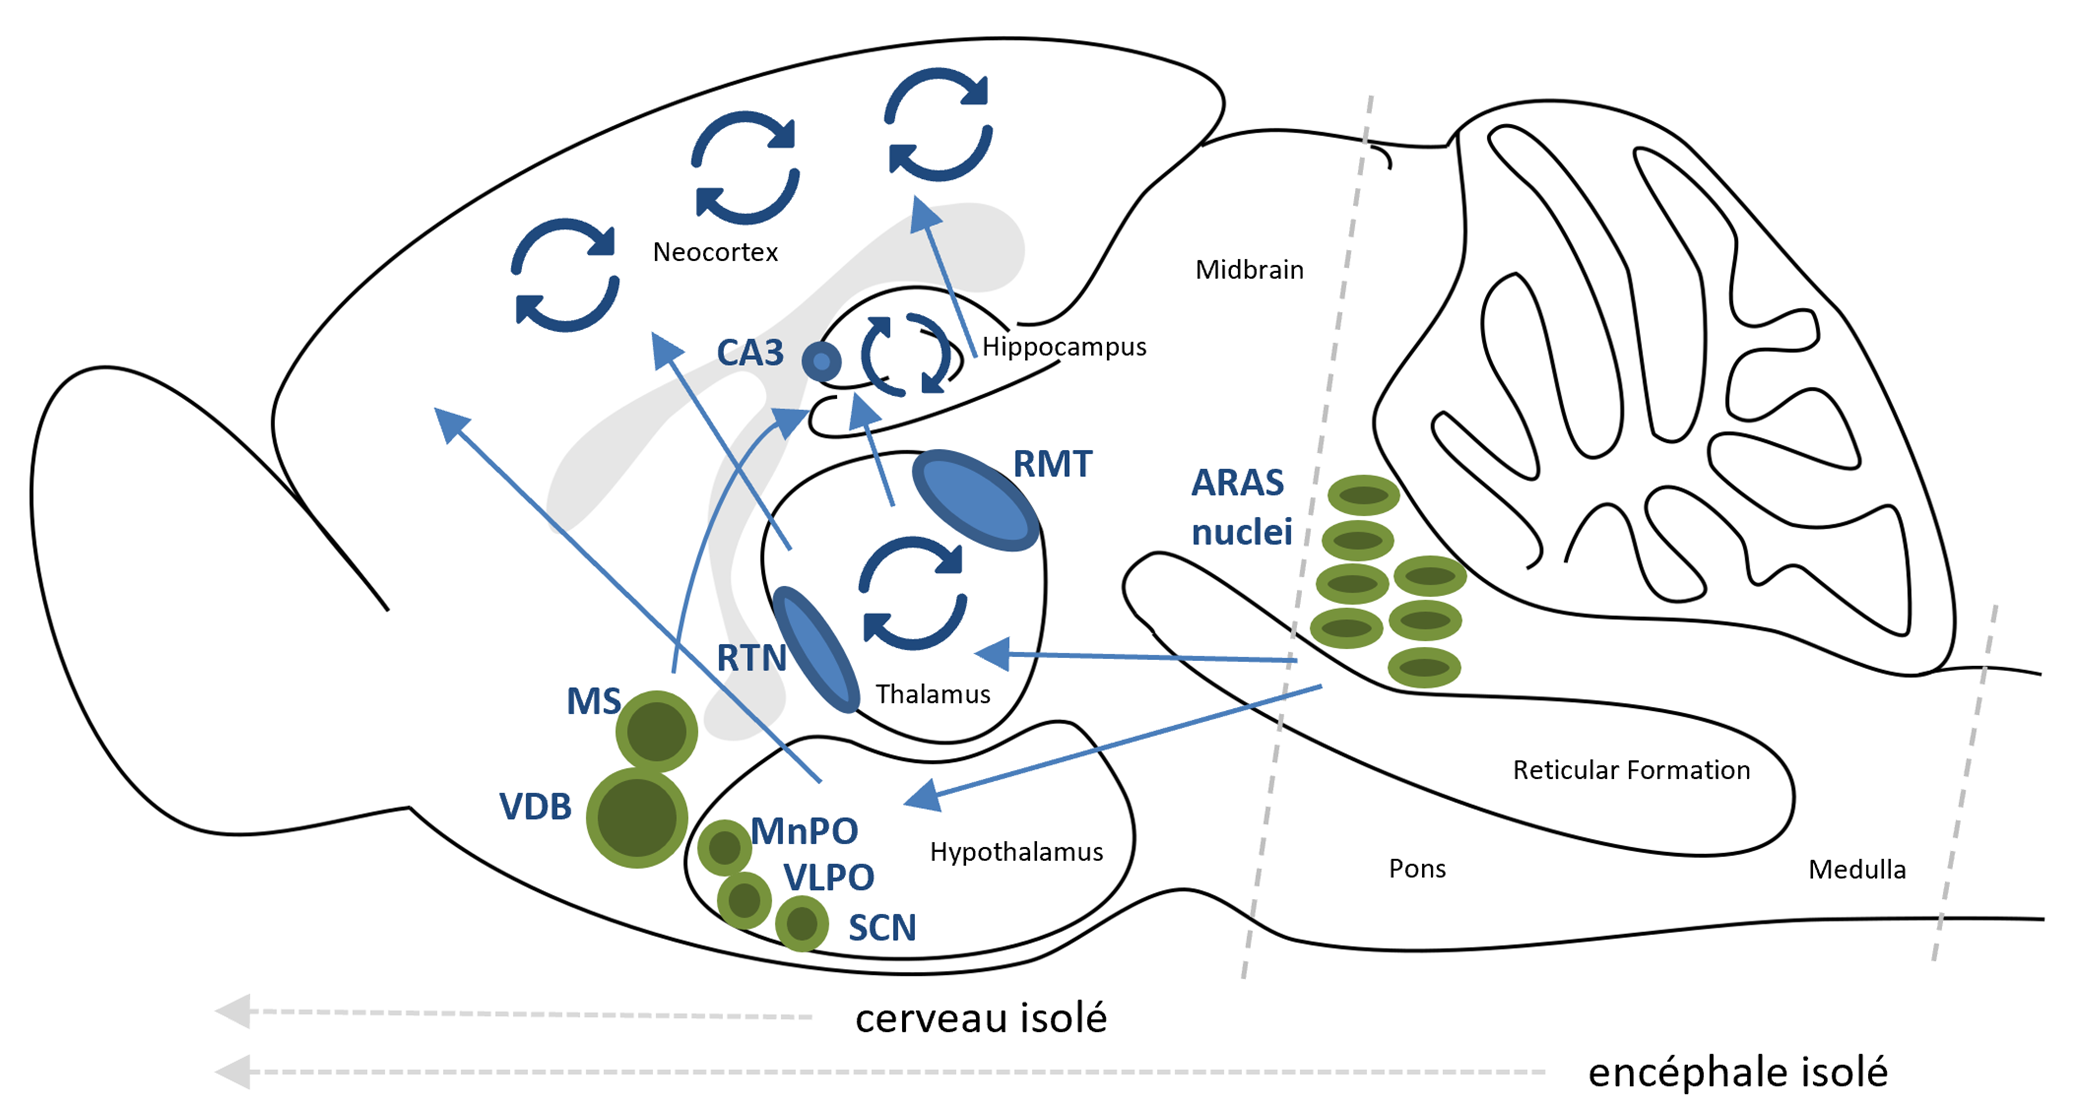
\includegraphics[width=\textwidth,height=\textheight,keepaspectratio]{Figures/oscillatory_centres_and_the_ascending_reticular_activation_system}
\decoRule
\caption[Oscillatory centres and the ascending reticular activation system]{Oscillatory centres and the ascending reticular activation system.\\
Circular arrows illustrate sites that act as neural oscillators. Thalamocortical slow waves in the delta range are assumed to originate from the lateral posterior nucleus of thalamus. Thalamocortical sleep spindles are produced in the reticular thalamic nucleus. Rostral midline thalamus (RMT) arguably acts as a relay for the ARAS and abolishes delta waves. It projects to cortex in a non-specific manner. Hippocampal sharp-wave-ripples arise in the subfield CA3 of hippocampus proper. Slow cortical oscillations (<1Hz) and high frequency waves arguably arise in neocortex. Straight arrows indicate the lateral and dorsal pathways of the ascending reticular activation system. Note that centres in the basal forebrain (BF) may suppress the generation of hippocampal short-wave-ripples. Arrows do not relate to the anatomical location of projection fibres and indicate no preferential sites within the target structure. The transections of the preparations “ceveau isolé” ad “encephalé isolé” are indicated by dotted lines. Slow waves occur in the cerveau isolé while normal sleep patterns have been observed for encephalé isolé. Abbreviations: Reticular thalamic nucleus (RTN), Lateral posterios nucleus (LP) Medial nucleus of the preoptic area MnPO and ventrolateral nucleus of the preoptic area (VLPO),  Basal forebrain including the
Medial septum (MS) and the Vertical Limb of the Diagonal Band (VDB), suprachismatic nucleus (SCN), rostral midline thalamus (RMT), Nuclei of the ascending reticular activation system (ARAS nuclei) including serotoninergic neurons in the raphe nucleus, norepinephrine neurons in locus coeruleus and glutamate neurons in the pedunculopontine nucleus. While oscillatory centres are isolated inter projections allow for interaction that can cause patterns to occur at the same time. Own depiction inspired by \parencite[1099]{brown2012control}.}
\label{fig:oscillatory_centres_and_the_ascending_reticular_activation_system}
\end{figure}
%-----------------------------------
%	SECTION 3.2
%-----------------------------------
\subsection{Neural oscillators and relays for ascending activation}
\label{ascending_system_and_oscillators}
Both the transition to the bistable state of slow wave sleep and fluctuations in the delta range include ascending signals that originate from subcortical areas. Several centres have been identified that generate oscillatory patterns of spiking activity. These patterns include (1) thalamocortical sleep spindles, (2) hippocampal sharp wave ripples (3) delta waves of thalamic origin and (4) neocortical slow waves. Distinct pacemakers exist which neural oscillators and cause named rhythms in the brain.\\

\textbf{Rostral midline thalamus: A relay for ascending activation}\\
The circumstance that slow waves were measurable in cerveau isolé preparations indicates that slow waves are initiated in brain regions above pons. Thalamus is considered a relay for ascending signals in the awake state. It shows that specific nuclei act as neural oscillators especially under certain conditions, most notably sleep. "During these states, the behavior of thalamic cells is characterized by long-lasting hyperpolarizations and phasic burst discharges recurring rhythmically" \parencite[p. 21]{steriade1984thalamus}. Chirurgical removal of thalamus in cats was found to lead to a decrease of the amount of non-REM sleep from 38\% to 11.8\%. In contrast diencephalic cats still showed sleep spindles \parencite{montagna2005fatal}. Further support comes for example from fatal familial insomnia. Findings indicate that thalamic atrophy causes a lack of sleep spindles and delta sleep which implies that "thalamus is the origin of slow wave sleep" \parencite[p. 339]{montagna2005fatal}.\\
Thalamic nuclei contain neurons that oscillate in the rhythms of slow waves highlighting its role for the regulation of sleep. Evidence suggests, however, that Rostral Midline Thalamus (RMT) acts as a relay for ascending arousal signals that originate from the reticular formation and abolish slow waves. Stimulation of the midbrain reticular formation in cats suppresses slow thalamic rhythms of hyperpolarizing episodes \parencite{steriade1984thalamus}. RMT is part of the nonspecific thalamic system. It contains nuclei that project to cortex in a spatially unspecific manner. While specific roles can be attributed to some cores one can assume RMT to alter the excitability of cortical neurons in a spatially rather unspecific way. \parencite{vertes2015limbic}. Phasic desynchronization of the neocortex could only be observed upon stimulation of the midline thalamic area in cerveau isolé preparations of cats \parencite{kawamura1968hippocampal}. Rostral midline thalamus relays signals of the ARAS that abolish slow waves.\\

\textbf{Lateral posterior nucleus: Source of delta oscillations}\\
While it was previously found that thalamic delta waves are absent in diencephalic cats where cortex is surgically separated from lower stuctures \parencite{villablanca2004counterpointing}, Dossi et. al \parencite*{dossi1992electrophysiology} identified thalamocortical slow waves in the posterior lateral posterior nucleus of thalamus (LPN) that show delta oscillations (here: 0.5 - 4 Hz) even after dissection of related cortical areas. Intracellular recordings show highly rhythmical oscillations in membrane potential at around 0.5 Hz. These oscillations occur spontaneously. When exceeding a certain threshold each of these oscillations was found to generate exactly one action potential at peak depolarization. Moreover, is showed that self-sustained delta oscillations can be elicited by electrical stimulation in short rhythmic pulses \parencite{dossi1992electrophysiology}. These findings (1) clearly indicate that LPN is a thalamocortical center that generates delta waves and (2) that rhythmical excitation entrains neurons to exhibit a delta rhythm.\\
More recently the T-type calcium channels have been found to play a key role in thalamocortical circuits that generate slow waves in the delta range. EEG delta waves are practically absent during NREM sleep in knockout mice that lack the alpha G1 subunit of named calcium channel. Moreover, the duration of NREM sleep is generally reduced \parencite{lee2004lack}. However selective modification of T-type calcium channels in RMT were found to have similar consequences \parencite{brown2012control}. This potentially indicates an abolishing effect due to changes in the thalamic relays of the ARAS.\\
As thalamic cores and cortex are strongly connected it can be argued that they represent a common functional unit for the generation of delta waves \parencite{crunelli2018dual}. The circumstance that rhythmical stimulation elicits delta waves indicates that interactions between oscillations in thalamus and cortex exist. Potentially they bind activity in thalamocortical networks. However, the oscillators that produce slow waves in the delta range rely in thalamus.\\

\textbf{Thalamic reticular nucleus: Generator for sleep spindles}\\
Another thalamic nucleus is considered the source of sleep spindles. Sleep spindles manifest as patterns of damped oscillations in EEG. Sleep spindles are well visible in the frequency band between 7 and 15 Hz \parencite{niethard2018cortical}. These patterns in EEG arguably arise from synchronous firing of cortical pyramidal cells. It is known however that sleep spindles originate from the thalamic reticular nucleus \parencite{luthi2014sleep}. Thalamocortical sleep spindles are considered to be a switch for the transition between light and deep sleep \parencite{montagna2005fatal}. In many cases they cooccur with activity of cortical cells measured by two photon fluorescence microscopy \parencite{niethard2018cortical}. The reticular thalamic nucleus is considered the pacemaker for sleep spindles that interact with slow waves.\\

\textbf{Hippocampal formation: Origin of sharp wave ripples}\\
Another area in the brain that is known to act as a neural oscillator resides in the hippocampal formation. Hippocampus represents the oldest part of cortex and exhibits a highly structured nature that has been extensively studied. An important feature of the organization of hippocampus is the overall flow of signals that follows the scheme of the tri synaptic way. Signals from entorhinal cortex travel in circular patterns through hippocampus. Activation propagates from entorhinal cortex to the dentate gyrus, subsequently to the CA3 subfield, via the Schaffer collaterals further to subfield CA1 and finally back to the entorhinal cortex. This network topology is incorporated in spiking neural networks that can reproduce important features of hippocampal sharp wave ripples \parencite{aussel2018detailed}.\\
Hippocampal sharp wave ripples can be produced in vitro. Long term potentiation of neurons that form the recurrent networks that include subfield CA3 is known to facilitate the generation of hippocampal sharp wave ripples. Repeated high-frequency stimulation of a particular area in subfield CA1 induces long term potentiation and enables short wave ripples both in area CA3 and CA1. These findings do not only indicate the source of origin of hippocampal sharp wave ripples but also its involvement in processes of memory formation \parencite{behrens2005induction}.\\

\textbf{Neocortex: Source of neocortical slow waves}\\
Neocortical slow waves occur spontaneously during deep sleep and deep anaesthesia in irregular rhythms with a frequency of one Hz and below. Differences have been found for ketamine induced anaesthesia and urethane where frequencies were found to be slightly lower \parencite{steriade1993novel}. Neocortical slow waves have been described as recurring bursts of action potentials of neurons in wide regions of cortex. Simultaneous acquisition of electrocorticograms (ECoG) shows that these bursts cooccur with an oscillation in the electrical potential on the cortical surface \parencite{steriade1993novel}. Arguably these oscillations relate to neocortical slow waves [< 1Hz] that can be measured using EEG during deep sleep. Simultaneous ECoG and widefield flouroscence imaging shows that up states typically cooccur with several oscillations of the ECoG potential (Stroh et al. \cite*{stroh2013making}; see figure 2.1). \\
Simultaneous recording of ECoG and local field potentials (LFP) in the form of a electrothalamigram indicates the presence of a corresponding thalamic signal \parencite{steriade1993novel}. The hypothesis that neocortex contains networks that act as a neural oscillator has been confirmed both empirically and by means of simulation (see section \ref{effects_of_anaesthesia}). However, it was also found that optical stimuli and the resulting signal that originates from the retina are suitable to elicit slow waves. Besides optogenetic stimulation of the lateral geniculate body, the thalamic relay for signals from the retina, causes slow waves. Neocortical slow waves can hence not only arise because of random noise that manifests as spontaneous firing but can also be triggered by perceptual inputs and excitatory projections from subcortical sites. Moreover, it was shown that slow waves evoked in cortex strictly precede a signal that can be measured in thalamus. \parencite{stroh2013making}. Taken together this indicates that cortex is the site of origin for this type of slow waves. Oscillations arise spontaneously while the interaction with other signals can arguably determine the precise time of the occurrence of neocortical slow waves.\\
Two photon fluorescence microscopy reveals a differential behaviour of different neurons during up states of slow wave anaesthesia. It shows that neurons do not all behave in the same way but peak activity cooccurs with sleep spindles only for some neurons. In average the fluorescence signal correlates with slow waves measured using ECoG. As mentioned above the electrophysiological response does however not directly reflect the df/f signal. Different neurons have specific response properties and cooccur with other oscillations in the brain in a selective manner (see also \ref{slow_waves_and_memory}).\\

\textbf{Interaction effects}\\
Interaction effects between signals that arise from thalamus and those in cortex have been identified. Thalamus is evidently the source of sleep spindles and delta waves, the most important patterns of slow wave sleep. However, it shall be mentioned that thalamus is strongly interconnected with cortex. Electrical stimulation of the reticular core of thalamus was found to cause an increased in amplitude of delta waves in hippocampus. In contrast rhythmical stimulation of cortical area 7 evokes periodic oscillations in thalamic neurons that sustain over extended periods of time after stimulation offset. The resulting thalamic rhythm can in return enhance synchronization \parencite[p. 21]{steriade1984thalamus}. This finding indicates not only that entrained rhythms exist in thalamus but also that oscillations in thalamus and both archicortex and neocortex strongly relate to each other.\\
Sleep spindles, hippocampal sharp wave ripples and neocortical slow waves are arguably not fully independent. Slow waves predominantly occur phase locked to sleep spindles \parencite{demanuele2017coordination}. The spindle amplitude is correlated (r = .3) with the df/f signal in wake active cells \parencite{niethard2018cortical}. A weaker yet significant correlation is found for wake inactive cells. The cooccurrence of slow oscillations and sleep spindles is also correlated with effects on the calcium fluorescence. A higher percentage change can be observed when both signals coincide as compared to the case of sleep spindles alone being present during a slow wave in calcium fluorescence \parencite{niethard2018cortical}. Contingencies between hippocampal sharp wave ripples and slow waves and the role they play for memory consolidation are discussed in the next section.\\
Neocortical slow waves can be perceptually triggered and evoked by optogenetic stimulation of subcortical areas. Stroh et al. \parencite*{stroh2013making} found that both the presentation of optical stimuli and optogenetic stimulation of the lateral geniculate nucleus (LGN) can cause neocortical slow oscillations. The LGN is the thalamic relay for visual information that originates from the retina and projects to visual area 1 (V1) in occipital cortex. The circumstance that slow waves can be triggered by signals that originate from areas other then cortex highlights potential interaction effects with other oscillations in the brain.\\
Figure\ref{fig:oscillatory_centres_and_the_ascending_reticular_activation_system} illustrates the location of oscillatory nuclei which evidently play a role in slow wave sleep and shows the ventral and dorsal pathway of the ascending reticular activation system. The SCN that arguably plays an important role in the regulation of sleep according to the circadian cycle is additionally indicated. Note that oscillatory centres in the rostral medulla that orchestrate breathing during sleep are not shown \parencite{kubin2019interactions}.\\
While the named structures are arguably the source of the respective oscillation it must be noted that signals interact. They do not occur fully independently. Up and down states of neocortical slow waves arise in cortex while they can be caused by subcortical afferences. Empirical data indicates that oscillations in archicortex and thalamus are more or less tightly bound to neocortical slow waves \parencite{niethard2018cortical}. The presumed role of cortico-hippocampal synchrony for memory consolidation is discussed in the next section.\\
%-----------------------------------
%	Section 4
%-----------------------------------
\section{Sleep slow waves and memory consolidation}
\label{slow_waves_and_memory}
A proposed function of slow waves is to "bind together" \parencite[1110]{brown2012control} several oscillatory patterns during sleep. Moreover, it was argued that slow waves represent an important mechanism for memory consolidation. According to the hippocampal-neocortical dialogue model of slow waves, the interaction of hippocampal sharp wave ripples and neocortical slow waves fosters memory consolidation \parencite{buzsaki1996hippocampo}: Recently it was shown that generating neocortical slow waves in prefrontal networks such that they are coupled to the occurrence of sharp wave ripples in the hippocampus increases the performance of rats in a memory task \parencite{maingret2016hippocampo}. Coherently, a correlation of slow wave activity and the brain-derived neurotrophic factor was found for humans \parencite{duncan2013concomitant}. Spontaneously occurring slow waves arguably play an important role for memory.\\
The hippocampo neocortical dialog model states that memory acquisition is a two-stage process. Accordingly (1) associations between sparse perceptual codes and the internal world are formed in hippocampus whereas (2) memory replay occurs during slow wave sleep and establishes long term memories in the interaction with neocortex. A further hypothesis states that information is gathered sequentially during theta oscillations and replay occurs during sharp wave population bursts \parencite{buzsaki1996hippocampo}. Important key elements of the model are well supported by empirical findings.\\
Entorhinal cortex represents the neocortical interface to hippocampus. It provides both the main input and is the main target area of hippocampal projections \parencite{buzsaki1996hippocampo}. Entorhinal cortex resides on the highest hierarchy level of the Van Essen Diagram \parencite{felleman1991distributed}. Visual information can be assumed to be processed in a hierarchical manner along the ventral pathway. Whereas response properties in early visual cortices relate to physical features of the visual percept such as simple shapes that occur in a specific receptive field, neurons evidently code for more abstract concepts in higher areas. Famous examples are the parahippocampal place area (PPA) or the fusiform face area (FFA) both of which reside in close proximity of the hippocampal formation \parencite{coggan2019selectivity}. It can be deemed certain that that hippocampus receives a highly processed perceptual code.\\
Hippocampus exhibits a well-defined structure that contrasts with neocortex and includes circular pathways of projections that allow for recurrent activity \parencite{graham2010associative}. Electrophysiological studies of hippocampal circuits revealed that long term potentiation occurs in hippocampus. High frequency stimulation causes long lasting effects highlighting the role of hippocampus for learning \parencite{behrens2005induction}. Simulation studies indicate that hippocampus acts as an auto associative memory \parencite{graham2010associative}. Strikingly specific protocols of high frequency stimulation were not only found to cause long term potentiation but have recently been shown to act as a trigger for hippocampal sharp waves \parencite{behrens2005induction}.\\
 While hippocampus plays an important role for the acquisition of memories it is known that neocortical sites encode learned contents \footnote{Only moderate effects of retrograde amnesia exist in patients with hippocampal lesions indicating that declarative memory formation but not retention is impaired \parencite{spiers2001hippocampal}. The performance of rats with hippocampal lesions is impaired both for spatial learning and novel object recognition tasks but not in motor skill learning \parencite{gould2002effects}.}. The entrainment of cortical sites by previously acquired hippocampal codes during sleep is postulated by the neocortical hippocampal dialogue model and can be demonstrated empirically.\\
Empirical data shows that memory replay occurs during sleep both in hippocampus and the associated cortical sites. Both areas contain neurons that code for the learning experience. Ji and Wilson \parencite*{ji2007coordinated} investigated contingencies between behaviour and slow wave sleep to study the interaction between hippocampus and neocortex in the acquisition of long term memories. They investigated the response properties of neurons in rats in an experimental paradigm that includes maze running in an eight shaped maze. Place cells were identified that fire for different regions of the maze. Depending on the direction of running different patterns in the neural response show. The sequence of peak activities of the recorded neurons codes for the direction in which the rat passes through the maze. It was found that these sequences are replayed in hippocampus during slow wave sleep. Most interestingly, however, memory replay did not only take place in archicortex but neocortical signals appeared to be correlated. Neocortical place cells were also active. Moreover the same sequences of neural responses are measurable in hippocampus and neocortex which indicates that memory replay occurs during deep sleep \parencite{ji2007coordinated}.\\
Evidence further suggests that the synchrony between slow waves and hippocampal sharp wave ripples during sleep enhances learning. This was demonstrated in a stimulation paradigm where slow waves are triggered such that they coincide with sleep spindles measured in the hippocampal formation \parencite{maingret2016hippocampo}. It is not fully understood why increasing the synchrony between two signals that can oscillate independently fosters memory consolidation. One may speculate, however, that hippocampal signals can change synaptic weights of neocortical populations only if they trigger action potentials. Hence a simultaneous up state would be required.\\
As hippocampal memory replay is associated with specific neocortical neurons one may hypothesize that signals such as sharp wave ripples could trigger slow waves that incorporate distinct populations which correspond to the learning experience. Memory consolidation would accordingly be achieved by strengthening the synaptic weights of (1) the memory engram in neocortex by repeated activation of the respective synapses and (2) the associations between these neurons and sparse hippocampal codes.\\
 As mentioned above source modelling of sleep slow waves indicates cingulate fibre trajectories \parencite{murphy2009source}. Hippocampus and entorhinal cortex where the fibers of cingulum originate rely in close proximity and are part of the Papez Loop \parencite{choi2019papez}. Hence one may speculate that this pathway contributes to the hippocampo neocortical dialogue. With its high spatial resolution fluorescence microscopy can provide more fine-grained distinctions and may potentially reveal trajectories of neural signal transduction during slow wave sleep and anaesthesia. This highlights the importance of methods that allow to capture the variations of temporospatial patterns of neural slow waves.\\
%-----------------------------------
%	Section 5
%-----------------------------------
\section{Neocortical slow waves: Towards a working definiton}
\label{working_definition}
A distinction between slower and shorter waves has already been made in the pioneering electroencephalographic study almost a century ago \parencite[p. 550]{berger1929}. Shortly later the term delta wave was coined to describe oscillations in the recorded voltage in the respective frequency band. Delta waves are defined for a frequency of 1 to 4 Hz by some authors \parencite{kubin2019interactions} while others define the delta range for oscillations between 0.5 to 4Hz \parencite{dossi1992electrophysiology}. The term slow wave is also used to describe oscillatory patterns in EEGs in the delta range. "Slow-wave activity (SWA) is defined as the EEG power in the slow wave frequency band" \parencite[p. 1]{furrer2019sleep}. It shows that the term "delta wave" is sometimes used as a synonym for "slow wave". The term slow wave is rather loosely defined, and it is hence important to give a clear account of what is understood as a slow wave here.\\
Slow waves refer to a pattern in EEG but also to distinct neural phenomena. Depending on the context slow waves describe as a pattern measured with one method or oscillations that can be recorded in a methodologically rather agnostic way. For example changes in the spike rates of neurons or fluorescence signals are also referred to as slow waves \parencite{jercog2017up, stroh2013making}. This shows that the term slow wave is used in relation to the neural phenomenom, its functions and its signatures that can be measured using various methods.\\
Slow waves in the wide sense are both neocortical slow waves and thalamocortical slow waves in the delta range. For example, Celotto et. al \parencite*{celotto2020analysis} denote neocortical slow oscillations as slow waves. Furrer et al. \parencite*{furrer2019sleep} use the term as a synonym for delta waves instead. As explained in the previous sections both phenomena can occur independently from one another. It is hence advisable to use distinct terms. Steriade et. al \parencite*{steriade1993novel} suggested the label neocortical slow oscillation. It was noted, however, that the up states and down stated do not necessarily appear in a rhythmical pattern \parencite{brown2012control}. In addition, the transition to an up state appears as a slow travelling wave. As the term is more descriptive this phenomenon is hence referred to as neocortical slow wave. In contrast thalamocortical slow waves relate to slow waves in the delta band (1-4 Hz). Sleep slow waves show more irregular patterns in EEG and could potentially include signatures of both neocortical slow waves and thalamocortical slow waves in the delta range \parencite{steriade1993novel}.\\
Slow waves are short periods of above baseline activity that occur in bistable states such as deep sleep and anaesthesia which are characterized by reduced neural activity. Slow waves relate to the periods of up states activity that are interlaced with down states \parencite{jercog2017up}. They are dynamic patterns of recurrent activation of large potentially distinct populations of neurons. Slow waves can differ with respect to the pathway of neural flow that shows especially in early stages and with respect to the set of recruited cells where recurrent activity prevails. They appear as propagating waves in widefield and two-photon calcium imaging in vivo \parencite{celotto2020analysis, niethard2018cortical}.\\
Slow waves are dynamic patterns of flow. The rising phase of slow waves can be understood as a runaway process: If activity exceeds the threshold they fire and cause postsynaptic potentials which can elicit action potentials in the target neurons \parencite{nghiem2018two}. Travelling waves can arguably be observed because of the spatial arrangement of neurons in cortex where close sites are preferably connected more strongly. Traveling waves can even be observed in neocortical slices in vitro \parencite{wu2008propagating}. Cortex is known to be of a highly recurrent nature \parencite{guamuanuct2017mouse}. Arguably this is why one can observe extended periods of activation as these neurons can be assumed to directly or indirectly project back to the ones that initially fired. Hence, slow waves can reveal regions of high functional connectivity. However also cingulate fibre trajectories were identified in EEG during sleep \parencite{murphy2009source}. Neocortical slow waves could also travel through cortex via structured fibre bundles. Patterns of neural flow could result from signals that travel via fibres of cingulum that connects entorhinal cortex and the bordering hippocampus with neocortical sites.\\
Neocortical slow waves can be understood as a process that includes synchronization with other neural oscillations. If hippocampal sharp wave ripples correlate with cortical up states one may speak of a hippocampo neocortical slow wave. Thalamocortical slow waves arguably interact with the networks that cause neocortical slow waves. Analogously one could form subcategorizations for slow waves that incorporate deviant sets of connected neurons.\\
The exact slow wave frequency depends on the method for data acquisition. Here data from widefield fluorescence imaging is analysed. This raises the question how slow oscillations in calcium imaging differ from their counterpart in EEG or ECoG. The simultaneous acquisition of ECoG and wide field GCaMP imaging reveals that up states cooccur with oscillations in the cortical potential. Slow waves in the mean fluorescence signal cooccur with slow waves in the electrophysiological recording \parencite{stroh2013making}. The respective correlation could also be demonstrated on the basis of individual cells using two photon imaging \parencite{niethard2018cortical}. It shall be noted however that the frequencies of neocortical slow waves differ between ECoG and widefield fluorescence. Lower frequencies could potentially be the result from smoothing due to lower sampling rates and the required exposure time in fluorescence imaging or an involvement of distinct populations of neurons at different points in time.\\
Slow waves can have several subsegments. Here slow waves are understood as short periods of above baseline activity. Hence they can incorporate multiple oscillations. These stages could potentially relate to distinct neural events. The circumstance that slow waves can include several oscillations is especially important for the detection and separation of events. It means, however, that events could not be separated based on local minima alone \parencite{celotto2020analysis}. Nonetheless, it is reasonable to assume that multi peak slow waves exist.\\
Conceptualizing slow waves as above baseline activity bears potentials for revealing the temporal dynamics of slow waves that incorporate several stages. It also means that new methods are required for the analysis the dynamic of slow waves. Slow waves can be defined in various ways. They are up states that may include several oscillations and have distinct properties that include dynamical pathways of flow and the synchrony with other oscillations in the brain.
\begin{figure}[!htb]
\centering
\includegraphics[width=\textwidth,height=\textheight,keepaspectratio]{Figures/ECoG_calcium_flourescence}
\decoRule
\caption[Frequencies of slow waves differ between measuring techniques]{Frequencies of slow waves differ between measuring techniques.\\
Data was recovered from supplementary figure 4A, Stroh et al. \parencite*{stroh2013making} for secondary analysis. Signals are smoothed using a gaussian filter and subsequently normalized. Baseline correction was applied for the calcium signal (lower left). The resulting noise reduced signals were investigated with respect to the frequencies present. Upper row: The normalized Electrocorticogram (left) and the frequencies power revealed by Fourier Transform (right). Lower row: The normalized signal change of the calcium response (left) and the corresponding frequency spectrogram (right). The frequency power is plotted in blue whereas a smoothed version is plotted in orange. It shows that the peak frequency of the hemodynamic signals relies below 0.2 Hz whereas the peak frequency of the calcium signal is above 0.7. Note also that slow waves of both signals are aligned but several ECoG oscillations occur during a hemodynamic event.\\
}
\label{fig:ECoG_calcium_flourescence}
\end{figure}

% Chapter Template

\chapter{Methods} % Main chapter title
\label{ChapterX} % Change X to a consecutive number; for referencing this chapter elsewhere, use \ref{ChapterX}



%----------------------------------------------------------------------------------------
%	SECTION 1
%----------------------------------------------------------------------------------------

\section{A new approach to track intracerebral bloodflow}
Typically GCaMP signals are recorded at a sampling rate of 25Hz \parencite{celotto2020analysis}. In contrast the dataset at hand was recorded at 100Hz. Highspeed recordings bear potentials for the analysis of neural signals beyond the frequency of neocortical slow waves. However, new methods must be established to identify what high frequency components relate to. This is especially important because widefield flouroscence recordings are confounded with an error that results from the hemodynamic autoflourescence. The results of a new approach indicate that high high frequencies in the df/f signal relate to particles of hemoglobin rich blood that flow through intracerebral bloodvessels of various size.\\
\begin{figure}[th]
\centering
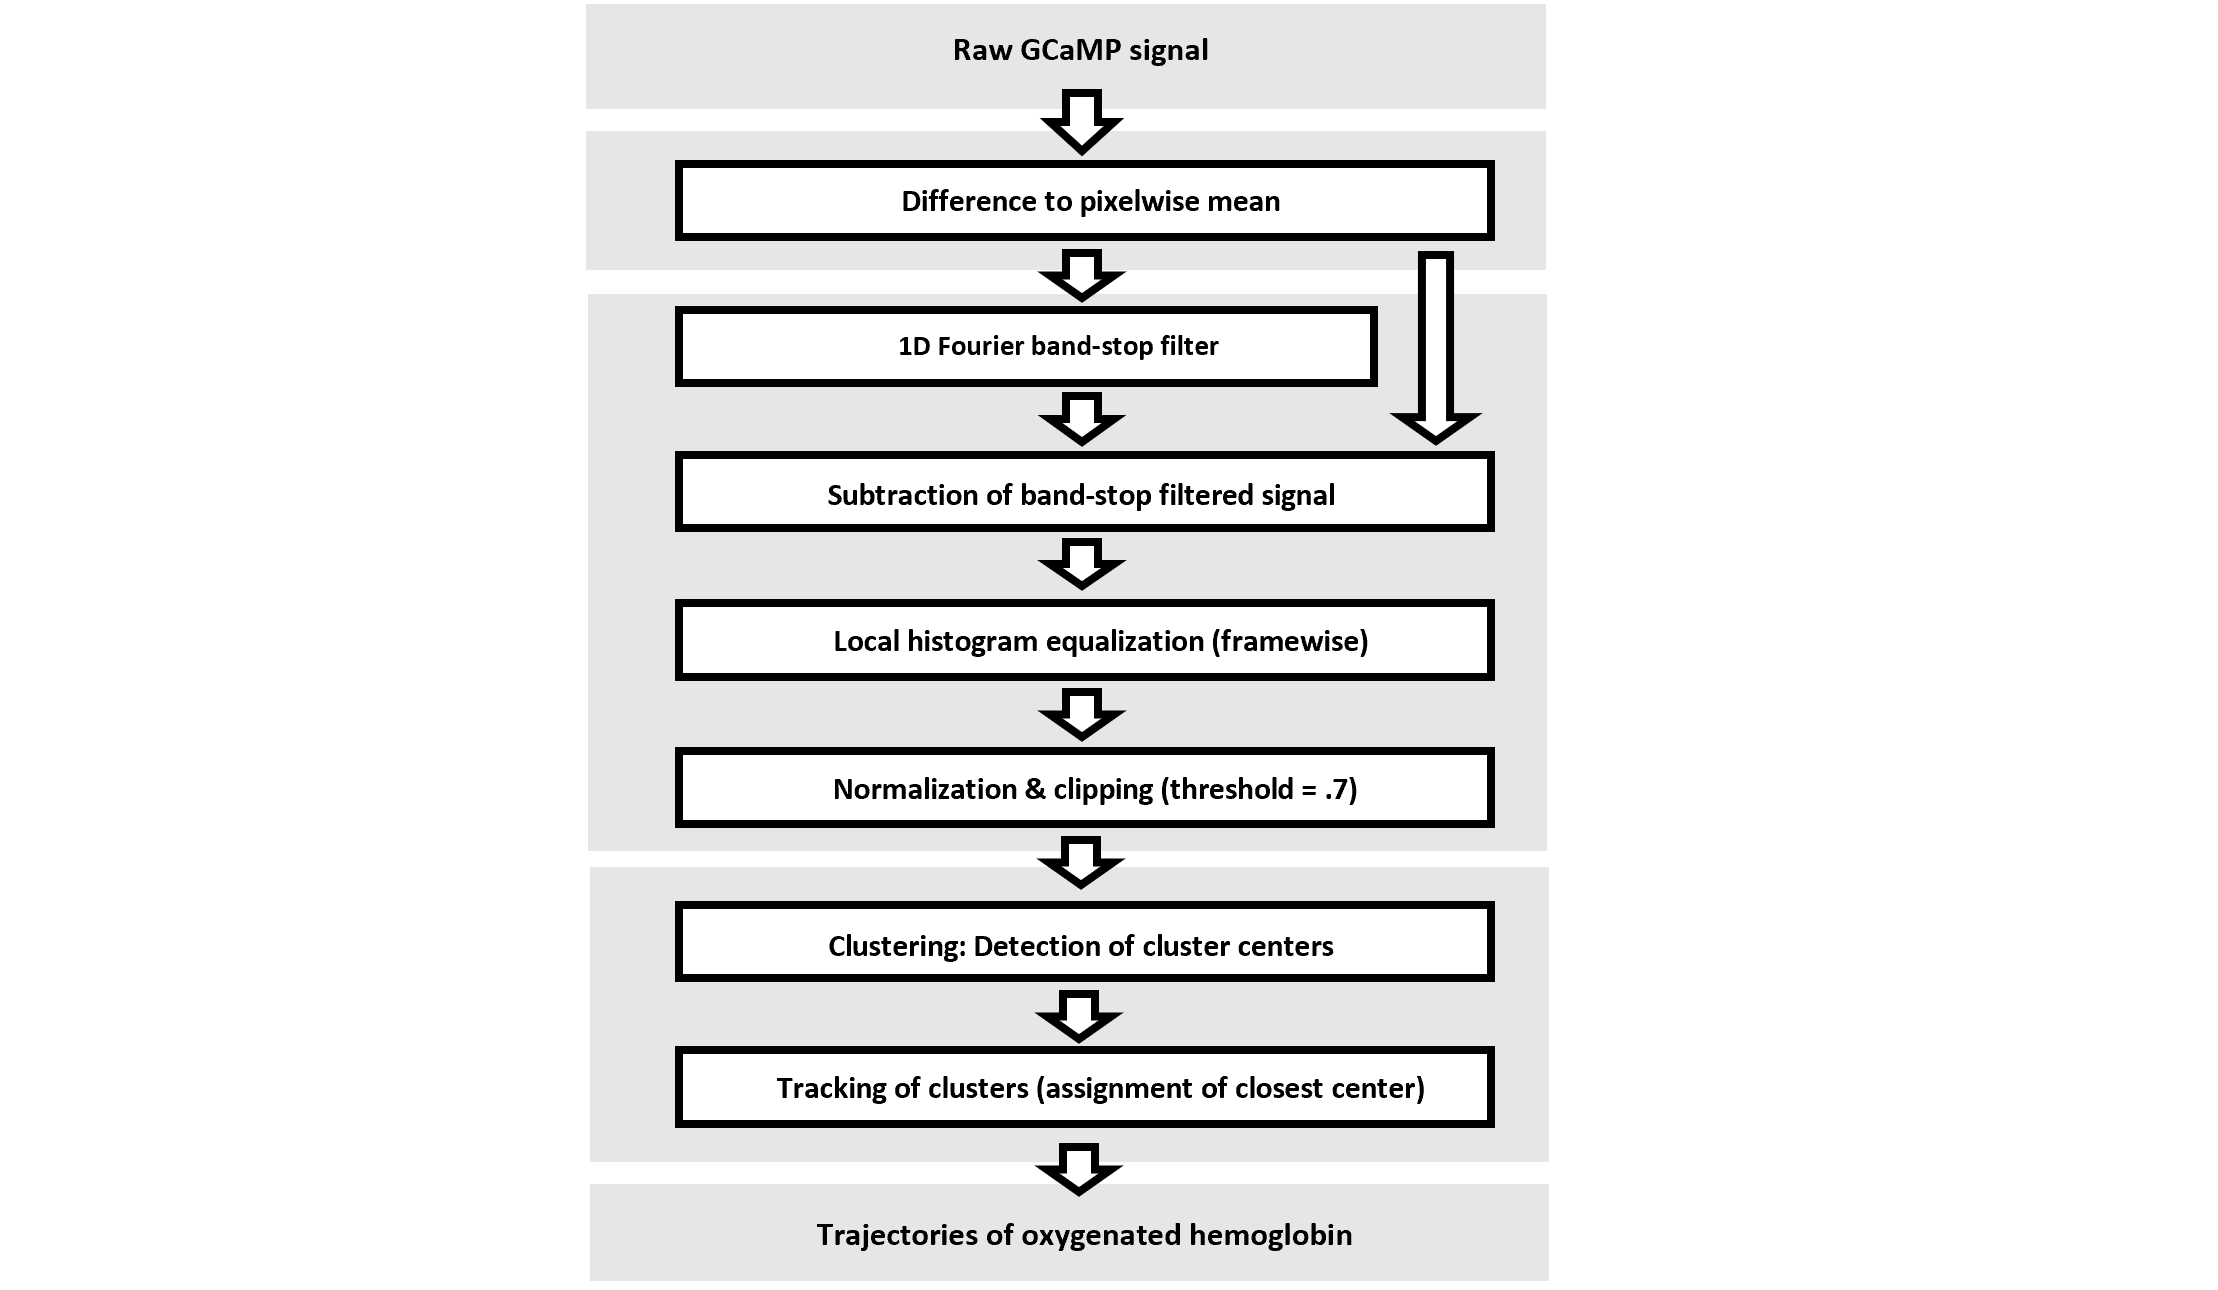
\includegraphics[width=\textwidth,height=\textheight,keepaspectratio]{Figures/tracking_bloodflow_pipeline}
\decoRule
\caption[Processing pipeline for the detection of bloodflow]{Processing pipeline for the detection of bloodflow}
\label{fig:clustering_approach_pipeline}
\end{figure}
\begin{figure}[th]
\centering
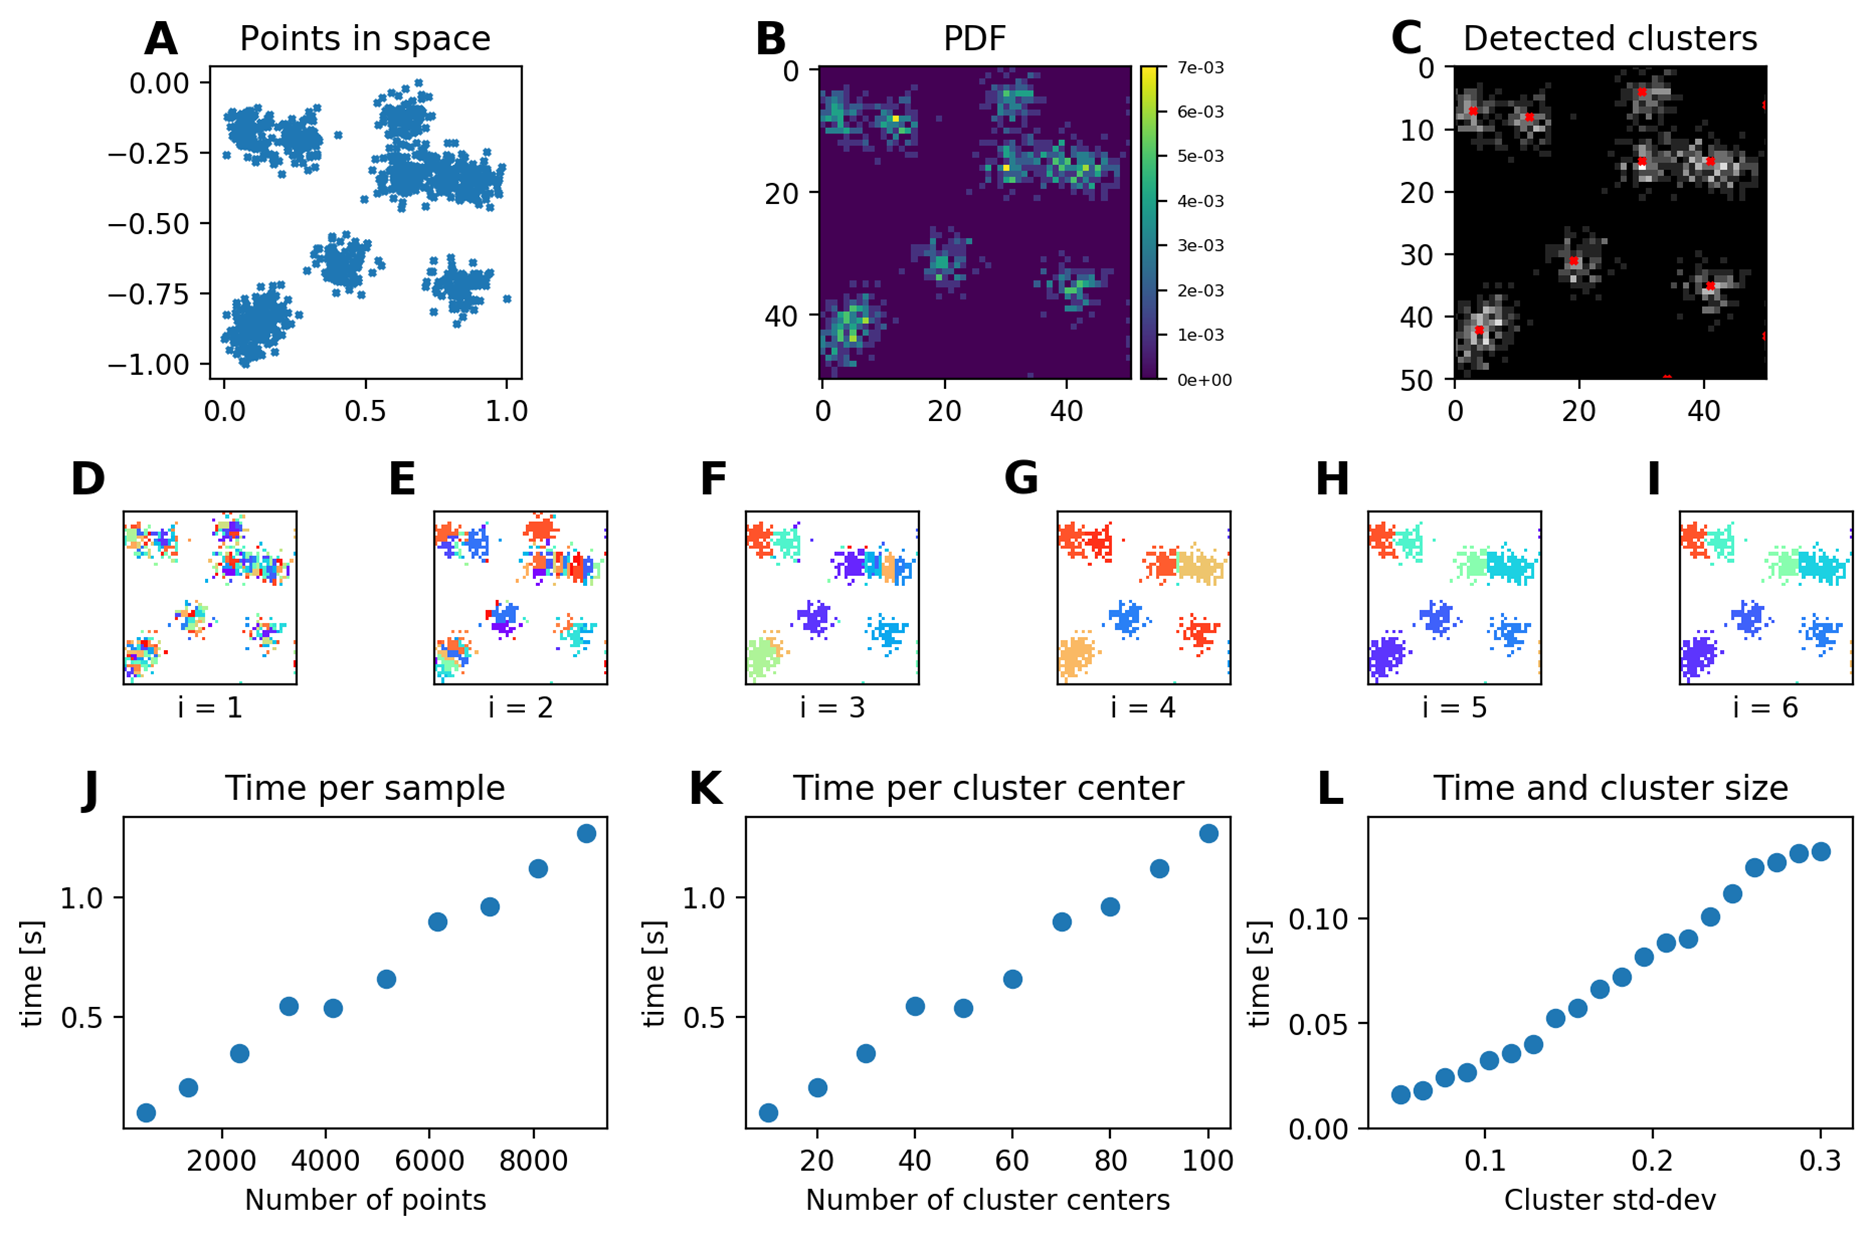
\includegraphics[width=\textwidth,height=\textheight,keepaspectratio]{Figures/clustering_approach_properties}
\decoRule
\caption[A mean shift approach for clustering pixels]{A mean shift approach for clustering pixels. After clipping the preprocessed hemodynamic signal, groups of bright, rather isolated foreground pixels are visible. These pixels can be considered as evidence for the presence of oxygenated hemoglobin particles. To detect the location of named clusters of pixels a variation of mean shift clustering was implemented that works with density matrices. Panel A: A distribution of points in $\mathbb{R^2}$. Cluster centers were sampled using a 2D gaussian. For each cluster center points were added using a second gaussian probability distribution centered at the respective location. Panel B : A 2D histogram of the distibution in panel A indicating the probability density function. Panel C: The detected cluster centers. Panels D-E: Assignment of pixels to clusters for the first seven iterations beginning with i=1. After iteration seven convergence is achieved. Panel J: Time per sample. Panel K: Time per cluster Panel L: Time per cluster size. }
\label{fig:clustering_approach_properties}
\end{figure}
\begin{figure}[th]
\centering
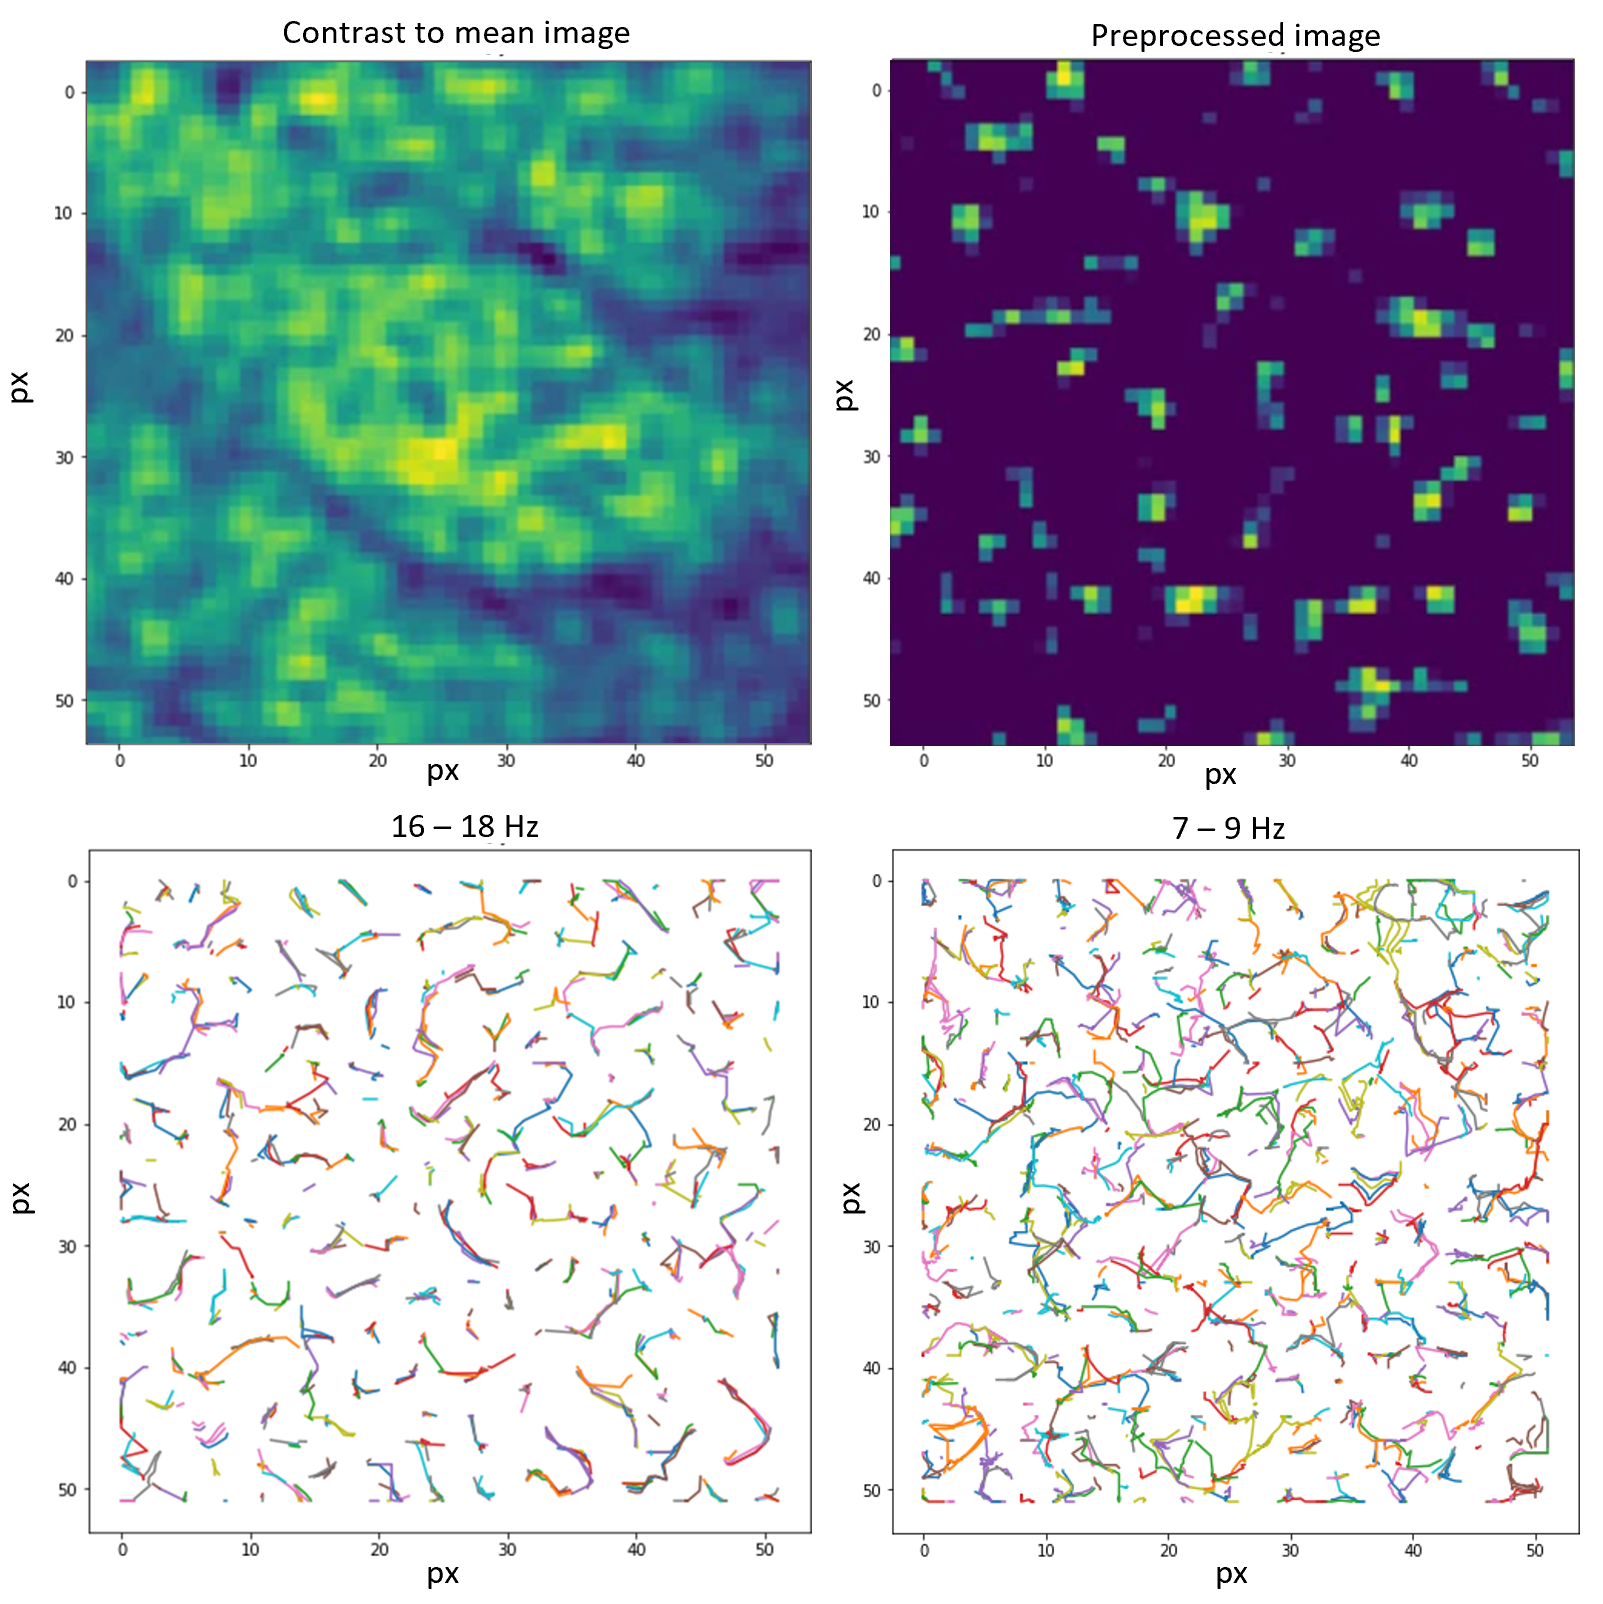
\includegraphics[width=\textwidth,height=\textheight,keepaspectratio]{Figures/clustering_approach_results}
\decoRule
\caption[Cluster tracking reveals trajectories of oxygenated hemoglobin]{Cluster tracking reveals trajectories of oxygenated hemoglobin.\\
Upper left: A sample frame for the original contrast to the pixelwise mean. Upper right: The preprocessed frame after application of clipping. Lower left: Detected trajectories for filtering of frequencies in the range of the heartbeat. Lower right: Detected trajectories of bloodflow for filtering of low frequencies. See also figure \ref{fig:clustering_approach_properties}}
\label{fig:clustering_approach_results}
\end{figure}
The approach presented here allows to measure intracerebral bloodflow without the need for the injection of tracers. Typically, microbeads are used to detect the flow rates and speed of intracerebral blood \parencite{kim2019development}. The study of intracranial bloodflow bears potentials for a better understanding of pathologic conditions and basic neurobiological functions of the brain. For example it was shown that the microvessel density decreases in brain tumors and characteristic chnages in the hemoglobin concentration can be observed \parencite{lee2014vivo}. However intracerebral bloodflow is also addressed in the neuroscience in the study of neurometabolic and neurovascular coupling \parencite{devor2012frontiers}. New approaches to track the bloodflow in the brain could help to better understand the interaction between the activity of neurons and bloodflow.\\
To determine what high frequency components of the flourescence signal relate to several processing steps were employed (see \ref{clustering_approach_pipeline}). First the mean image was calculated and subtracted from each frame of the recorded videos. The signal in time for each pixel was then bandstop filtered and the difference to the original signal was calculated. Bandstop filtering was achieved by tranforming the vectors to the fourier domain and setting the frequency components in the desired range to zero before applying inverse fourier transform. Adaptive histogram equalization was used to improve the contrast of each frame after clipping all values below a given threshold. In the resulting videos clusters of bright foreground pixels move on decisive trajectories (see figure \ref{fig:clustering_approach_results}).\\
Cluster tracking is used to measure the pathways of these temporospatial patterns. Objects in binary images that are potentially connected are oftenly labeled using watershed distance transform \parencite{arganda-carreras2016distance} \footnote{Distance transform assigns the value to the closest background pixel to each foreground pixel. Different algorithms exist that allow for fast approximations. The resulting image represents a heightmap if the distance values are interpreted as depth. A simple flooding algorithm can be used to determine the watersheds: A simulated rise of the water level fills basins in the heightmap. The borders between adjecent basins are the watersheds that seperate the detected objects.}. As the data was (1) not binarized but clipping was used and (2) has a low relative resolution which results in a rough outline does not allow for the computation of meaningful watersheds a different approach was used to detect clusters of connected foreground pixels. This approach represents a mean shift technique. \\
The clipped images were interpreted as probability density functions that indicate the presence of oxygenated hemoglobin. Clusters are detected by iteratively moving the density at a given location towards the center of gravity of a patch around this location. The algorithm stops if convergence is achieved or a maximal number of iterations is reached. The environment could be a squre or a circular patch. The impact could be weigthed using a 2D gaussian kernel to reduce the impact of distant points on the center of gravity. For the results shown in figure \ref{fig:clustering_approach_results} a simple rectangular patch was used. \\
Important properties were studied with simulated data. Figure \ref{fig:clustering_approach_properties} summarizes the results. The computation of 2D histograms can be achieved in o(n) as iterating over the data once is sufficient. As the size of this histogram can be chosen freely the computatio time does not directly depend on the number of samples. In the simulation data for each cluster was sampled using the same 2D gaussian with a given standard deviation. Given that convergence can be achieved it can hence be assumed that in average the algorithm takes the same amount of time for each cluster. The simulation confirmed a linear relationship (\ref{fig:clustering_approach_properties}K). Increasing the number of samples per cluster center also scales linearly with the processing time. A different picture shows for variations of the standard deviation of the cluster centers. A nonlinear relationship can be assumed.\\
Clustering was performed for each frame seperately. Tracking was achieved by assigning the closest cluster center of the subsequent frame (maximal distance 10 px). It shows that particles move on decisive trajectories. Deviant results can be achieved for different frequencies. If bandstop filtering is applied in the range of the heart rate shorter trajectories are detected. The clusters appeared to be larger indicating bloodflow in bigger vessels. In contrast for smaller vessels a more filigree pattern can be observed. It can be hypothesized that these patterns relate to blood that travels at different speeds in vessels of different size.

%----------------------------------------------------------------------------------------
%	SECTION 1
%----------------------------------------------------------------------------------------
\section{Dense Optical Flow}

Lorem ipsum dolor sit amet, consectetur adipiscing elit. Aliquam ultricies lacinia euismod. Nam tempus risus in dolor rhoncus in interdum enim tincidunt. Donec vel nunc neque. In condimentum ullamcorper quam non consequat. Fusce sagittis tempor feugiat. Fusce magna erat, molestie eu convallis ut, tempus sed arcu. Quisque molestie, ante a tincidunt ullamcorper, sapien enim dignissim lacus, in semper nibh erat lobortis purus. Integer dapibus ligula ac risus convallis pellentesque.

\section{Helmholtz-Decomposition}

\section{Helmholtz-Decomposition of Dense Optical Flow}

\section{The processing pipeline}
Widefield flouroscence microscopy makes use of slective differences in the reflectance of light of a specific wavelength that results from conformational changes of ion channels in the neural membrane. This approach is challanged by the hemodynamic autoflourescence due to the blood oxygen level. The flouroscence of oxygenated and deoxigenated hemoglobin depends on the frequency of the light used for illumination. At a wavelength of 405nm the differences are marginal. Nonetheless a hemodynamic error signal remains in the data. Fluctuations are especially visible in recordings with 100 Hz sampling rate as it is high enough to capture potential fluctuations in the flourescence due to breathing and the heartbeat. This is especially relevant for for deep anaesthesia as the GCaMP signal to hemodynamic noise ratio is higher.\\

% Chapter Template

\chapter{Results} % Main chapter title

\label{Chapter4} % Change X to a consecutive number; for referencing this chapter elsewhere, use \ref{ChapterX}

%----------------------------------------------------------------------------------------
%	SECTION 1
%----------------------------------------------------------------------------------------

\section{Main Section 1}

Lorem ipsum dolor sit amet, consectetur adipiscing elit. Aliquam ultricies lacinia euismod. Nam tempus risus in dolor rhoncus in interdum enim tincidunt. Donec vel nunc neque. In condimentum ullamcorper quam non consequat. Fusce sagittis tempor feugiat. Fusce magna erat, molestie eu convallis ut, tempus sed arcu. Quisque molestie, ante a tincidunt ullamcorper, sapien enim dignissim lacus, in semper nibh erat lobortis purus. Integer dapibus ligula ac risus convallis pellentesque.

%-----------------------------------
%	SUBSECTION 1
%-----------------------------------
\subsection{Subsection 1}

Nunc posuere quam at lectus tristique eu ultrices augue venenatis. Vestibulum ante ipsum primis in faucibus orci luctus et ultrices posuere cubilia Curae; Aliquam erat volutpat. Vivamus sodales tortor eget quam adipiscing in vulputate ante ullamcorper. Sed eros ante, lacinia et sollicitudin et, aliquam sit amet augue. In hac habitasse platea dictumst.

%-----------------------------------
%	SUBSECTION 2
%-----------------------------------

\subsection{Subsection 2}
Morbi rutrum odio eget arcu adipiscing sodales. Aenean et purus a est pulvinar pellentesque. Cras in elit neque, quis varius elit. Phasellus fringilla, nibh eu tempus venenatis, dolor elit posuere quam, quis adipiscing urna leo nec orci. Sed nec nulla auctor odio aliquet consequat. Ut nec nulla in ante ullamcorper aliquam at sed dolor. Phasellus fermentum magna in augue gravida cursus. Cras sed pretium lorem. Pellentesque eget ornare odio. Proin accumsan, massa viverra cursus pharetra, ipsum nisi lobortis velit, a malesuada dolor lorem eu neque.

%----------------------------------------------------------------------------------------
%	SECTION 2
%----------------------------------------------------------------------------------------

\section{Main Section 2}

Sed ullamcorper quam eu nisl interdum at interdum enim egestas. Aliquam placerat justo sed lectus lobortis ut porta nisl porttitor. Vestibulum mi dolor, lacinia molestie gravida at, tempus vitae ligula. Donec eget quam sapien, in viverra eros. Donec pellentesque justo a massa fringilla non vestibulum metus vestibulum. Vestibulum in orci quis felis tempor lacinia. Vivamus ornare ultrices facilisis. Ut hendrerit volutpat vulputate. Morbi condimentum venenatis augue, id porta ipsum vulputate in. Curabitur luctus tempus justo. Vestibulum risus lectus, adipiscing nec condimentum quis, condimentum nec nisl. Aliquam dictum sagittis velit sed iaculis. Morbi tristique augue sit amet nulla pulvinar id facilisis ligula mollis. Nam elit libero, tincidunt ut aliquam at, molestie in quam. Aenean rhoncus vehicula hendrerit.
% Chapter Template

\chapter{Discussion} % Main chapter title
%----------------------------------------------------------------------------------------
%	SECTION 1
%----------------------------------------------------------------------------------------
In summary, the combination of Optical Flow, Helmholtz Decomposition and Autoencoders allows to quantify important features of neocortical slow waves and reveals a complex topology of events in latent space. The approach has proven to be viable for the suggested event related analysis. However, improvements regarding the estimate of the df/f signal are necessary and the origin of a breathing related oscillations must be more closely examined. An event related analysis of neocortical slow waves and the use of VAEs on sparse features helps to distinguish different kinds of neocortical slow waves.\\
As the literature review showed, neocortical slow waves can originate in cortex spontaneously. However, they can not only be assumed to play an important role for memory but also to interact with other rhythms in the brain. Neocortical slow waves can be observed during bistable states of anaesthesia and deep sleep where both periods of recurrent activity and quiescence can be observed. Isoflurane induces a decrease in the junctional conductivity. Down states are arguably caused by Ca2+ accumulation that triggers Ca2+ gated K+ channels and leads to a population level refractory period \parencite{neske2016slow}. Neocortical slow waves can be triggered by subcortical stimulation \parencite{stroh2013making}. They typically incorporate only a subset neurons in cortex with strong interprojections. Arguably this explains why distinct areas of recurrent activity and decisive patterns of flow can be observed during different events.\\
Optical Flow and Helmholtz decomposition can help to measure pathways of flow and the centers of recurrent activity such that different types of events can be distinguished. It can hence be used as an alternative to approaches that detect the movement of wavefronts. Gradient based methods for Dense Optical Flow yield dense vector fields of displacement vectors for levelset boundaries (see section \ref{chapter_optical_flow}). This allow to measure more complex patterns which is especially important for neocortical slow waves with extended up states that exhibit a complex dynamic. These patterns of flow cannot be sufficiently described by moving wavefronts. Focal areas of brightness increase reflect areas of functional connectivity, manifest as sources in the vector fields and can be distinguished from patterns in the flow using Helmholtz decomposition (see section \ref{section_helmholtz_decomposition}). \\
Variational Autoencoders with two dimensional latent layers appear as a good choice for dimension reduction because the latent space distributions could easily be interpreted. Manifolds of reconstructions can be computed for points on an evenly spaced grid using the decoder (see section \ref{section_autoencoders}). This allows to reduce the dimensionality of the data and present it in a way that is intuitively understandable by the reader. Of the three models implemented here, the mixed input Autoencoder allows to distinguish events in the most fine-grained manner.\\
In general, it shows that the amplitude of events decreases with the dosage of anaesthesia. The flow-component of the vector fields retrieved with the Horn and Schunck method reveal a complex dynamic of events. Different types of slow waves can be distinguished in the latent space distributions that Autoencoders reveal. Large amplitude waves either refer to medial axis events or events that incorporate frontal regions as sources.\\
Medial axis events typically include RSD and secondary motor areas, in some cases, show decisive upwards flow. Occipito-frontal flow occurs especially in an early stage. In later stages of some events medial lateral flow can dominate and wide regions of the frontal lobe can act as centers of recurrent activity that include primary motor areas. As the mixed input Autoencoder shows, slow waves with sources close to the medial axis exhibit a trend towards upwards flow. However, the strongest flow can also occur in horizontal direction or in all four main directions. This arguably reflects the described spread from medial to lateral or a complex dynamic of flow patterns respectively. Medial axis events typically have a single peak with a steep rise and decline. The circumstance that RSD is involved leaves room for the hypothesis that also the neighbouring hippocampus might play a role. Cingulate fibers originate from entorhinal cortex which is also closely connected \parencite{milczarek2018spatial}. Respective trajectories in human EEG have been reported \parencite{murphy2009source}. The explanation that these events represent hippocampo neocotical slow waves is, however, only one possible explanation. Bottom up events could also be triggered by visual input to occipital cortex. Arguably, further research is necessary to explain the origin of this kind of neocortical slow waves.\\
The second type of large amplitude waves incorporates frontal to fronto-parietal sources. In some cases, downwards flow is stronger then flow in other directions. Typically however, flow in all main directions occurs. This arguably reflects the complex dynamic of this type of slow waves that, in many cases, incorporates multiple peaks. Frontal areas have also been reported to be the main sources of slow waves in humans \parencite[p. 1110]{brown2012control}. Neocortical slow waves with multiple peaks that reflect extended upstates occur predominantly during light anaesthesia.\\
Low amplitude events occur at higher levels of isoflurane. One type of low amplitude wave shows mainly frontal sources and has a second peak that is correlated with the hemodynamic breathing signal. This can be interpreted as evidence for neocortical slow waves that are synchronized with breathing. It is unclear, however, whether the breathing synchronized peaks reflect a hemodynamic effect or also relate to neural oscillations that occur simultaneously. The analysis of low amplitude slow waves also shows events that have sources in the barrel fields. As they process signals from the whiskers it appears possible that breathing coupled sensory input exist. Arguably further research is necessary to study the interaction between neocortical slow waves and breathing. As the effect of breathing correlated components is negligible at anaesthesia levels with a better signal to noise ratio it is advisable to employ the proposed approach for the respective conditions.\\
The signal to noise ratio at high levels of anaesthesia represents a challenge. In addition, a difficulty arises from the circumstance that the standard deviation of the detrended hemodynamic signal increases for higher levels of isoflurane. Moreover, the GCaMP signal decreases in strength in these conditions. This means that the experimental conditions are systematically confounded with a potential error signal.\\
Additional refinements in the preprocessing might be necessary to further reduce possible artifacts due to hemodynamic effects. Subtracting a regression fit has proven difficult as the hemodynamic signal for a given pixel showed to be only marginally correlated with the GCaMP signal. Potentially this is the case because a breathing synchronized neural oscillation coincides with the peaks in the hemodynamic signal. Whether this is the case could however not be finally answered. Named challanges limit the interpretability of the results achieved for high levels of anaesthesia. Using the approach to characterize slow waves for conditions where the signal to noise ratio is high can help to avoid potential problems.\\
Other improvements can be made with respect to the computation of the df/f signal. Instead of computing a contrast to the temporal mean per event one may compute the contrast to the temporal mean of down state frames. This strategy worked well for high signal to noise conditions with decisive down states. The way to compute the df/f that was used here was found to yield highly similar results. Although refinements in the preprocessing might be necessary, the approach is considered a valid method to analyze slow waves in flouroscence recordings. It allows to study neocortical slow waves using widefield fluorescence imaging.\\
Optical Flow, Helmholtz Decomposition and Autoencoders can be used to characterize slow waves. This bears multiple potentials for the analysis of neocortical events that occur under anaesthesia. As widefield fluorescence microscopy is challenged by the hemodynamic autofluorescence it is advisable to select stages of anaesthesia where neocortical slow wave occur with a good signal to noise ratio and to employ methodological triangulation: The use of fluorescence microscopy in combination with electrophysiological recordings has previously been shown to help in the interpretation of the results. The approach shown here could in principle even be used with ECoG or EEG. In future Optical Flow, Helmholtz Decomposition and Autoencoders can be used to characterize neocortical slow waves and put their properties into perspective with effects of anaesthetics. However the approach could also be used to study other contingencies as well as sleep slow waves. As sleep slow waves are thought to foster memory consolidation one may put fourth the hypothesis that different types of events exist which reflect the interaction between hippocampal sharp waves and neocortical slow waves. Optical Flow, Helmholtz Decomposition and Autoencoders can be used to study neocortical slow waves during sleep and anaesthesia using widefield flouroscence imaging or electrophysiological methods.


%----------------------------------------------------------------------------------------
%	THESIS CONTENT - APPENDICES
%----------------------------------------------------------------------------------------

\appendix % Cue to tell LaTeX that the following "chapters" are Appendices

% Include the appendices of the thesis as separate files from the Appendices folder
% Uncomment the lines as you write the Appendices

%% Appendix A

\chapter{Frequently Asked Questions} % Main appendix title

\label{AppendixA} % For referencing this appendix elsewhere, use \ref{AppendixA}

\section{How do I change the colors of links?}

The color of links can be changed to your liking using:

{\small\verb!\hypersetup{urlcolor=red}!}, or

{\small\verb!\hypersetup{citecolor=green}!}, or

{\small\verb!\hypersetup{allcolor=blue}!}.

\noindent If you want to completely hide the links, you can use:

{\small\verb!\hypersetup{allcolors=.}!}, or even better: 

{\small\verb!\hypersetup{hidelinks}!}.

\noindent If you want to have obvious links in the PDF but not the printed text, use:

{\small\verb!\hypersetup{colorlinks=false}!}.

%\include{Appendices/AppendixB}
%\include{Appendices/AppendixC}

%----------------------------------------------------------------------------------------
%	BIBLIOGRAPHY
%----------------------------------------------------------------------------------------

\printbibliography[heading=bibintoc]

%----------------------------------------------------------------------------------------

\end{document}
